% !TeX spellcheck = sl_SI
\documentclass[mat1]{fmfdelo}
% \documentclass[fin1]{fmfdelo}
% \documentclass[isrm1]{fmfdelo}
% \documentclass[mat2]{fmfdelo}
% \documentclass[fin2]{fmfdelo}
% \documentclass[isrm2]{fmfdelo}
\usepackage{graphicx}
\usepackage{subcaption}
\usepackage{tikz-cd}
\usepackage[utf8]{inputenc}
\usepackage[T1]{fontenc}
\usepackage{lmodern}
\usepackage{amsmath}
\usepackage{amsthm}
\usepackage{amsfonts}
\usepackage{amssymb}
\usepackage{enumitem}
\usepackage{commath}
\usepackage{mathtools}
\usepackage{adjustbox}
\usepackage{setspace}
\usepackage{bigints}
\usepackage{mathrsfs}

\makeatletter
\DeclareRobustCommand{\sqcdot}{\mathbin{\mathpalette\morphic@sqcdot\relax}}
\newcommand{\morphic@sqcdot}[2]{%
\sbox\z@{$\m@th#1\centerdot$}%
\ht\z@=.33333\ht\z@
\vcenter{\box\z@}%
}
\makeatother
\makeatletter
\DeclareRobustCommand{\k}{
    \mathcal{K}
}
\makeatletter
\DeclareRobustCommand{\h}{
    \mathcal{H}}
\makeatletter
\DeclareRobustCommand{\si}{
    \bar{\sigma}}
\DeclareMathOperator*{\supp}{supp}
\DeclareMathOperator*{\htt}{ht}
\makeatletter
\DeclareRobustCommand{\pot}{
    $\h-$pot
}
\graphicspath{ {./slike/} }


% naslednje ukaze ustrezno napolnite
\avtor{Filip Bezjak}
\naslov{Minimalni končni modeli prostorov}
\title{Minimal finite models}

% navedite ime mentorja s polnim nazivom: doc.~dr.~Ime Priimek,
% izr.~prof.~dr.~Ime Priimek, prof.~dr.~Ime Priimek
% uporabite le tisti ukaz/ukaze, ki je/so za vas ustrezni
% \mentor{izr.~prof.~dr.~Ime Priimek}
\mentor{dr. Petar Pavešić}
%\somentorica{doc.~dr.~Ime Priimek}
% \mentorja{}{}
% \mentorici{}{}

\letnica{2023} % leto diplome

%  V povzetku na kratko opišite vsebinske rezultate dela. Sem ne sodi razlaga organizacije dela --
%  v katerem poglavju/razdelku je kaj, pač pa le opis vsebine.
\povzetek{Za končni topološki prostor $F$ rečemo, da je končni model prostora $X$, če obstaja šibka homotopska ekvivalenca $f\colon X \rightarrow F$. Model je minimalen, če ima izmed vseh modelov najmanjšo kardinalnost. Končnim $T_0$ topološkim prostorom lahko priredimo simplicialne komplekse. Eden izmed glavnih izrekov v delu nam pa pove, da je geometrijska realizacija tega kompleksa šibko homotopsko ekvivalentna začetnemu prostoru. S tem dobimo orodje za iskanje končnih modelov prostorov. V tem delu bomo poiskali minimalne modele topoloških sfer in končnih grafov.}

%  Prevod slovenskega povzetka v angleščino.
\abstract{We say that a finite topological space is a model of a topological space if they are weak homotopy equivalent. A model is minimal if it has the smallest cardinality of all models of a space. Every finite $T_0$ space has its associated simplicial complex. One of the main theorems of this graduate thesis states that the geometric realization of the associated simplicial complex is weak homotopy equivalent to the initial space. This gives us a tool to find finite models of spaces. In this thesis, we will find minimal models of topological spheres and finite graphs.}

% navedite vsaj eno klasifikacijsko oznako --
% dostopne so na www.ams.org/mathscinet/msc/msc2010.html
\klasifikacija{55U10}
\kljucnebesede{Končen topološki prostor, šibka homotopska ekvivalenca, homotopska ekvivalenca, delno urejena množica, simplicialni kompleks, graf, sfera} % navedite nekaj ključnih pojmov, ki nastopajo v delu
\keywords{Finite topological space, weak homotopy equivalence, homotopy equivalence, partialy ordered set, simplicial complex, graph, sphere} % angleški prevod ključnih besed

\zapisiMetaPodatke  % poskrbi za metapodatke in veljaven PDF/A-1b standard

% aktivirajte pakete, ki jih potrebujete
% \usepackage{tikz}

% za številske množice uporabite naslednje simbole
\newcommand{\R}{\mathbb R}
\newcommand{\N}{\mathbb N}
\newcommand{\Z}{\mathbb Z}
\newcommand{\Sus}{\mathbb S}


% matematične operatorje deklarirajte kot take, da jih bo Latex pravilno stavil
% \DeclareMathOperator{\conv}{conv}
% na razpolago so naslednja matematična okolja, ki jih kličemo s parom
% \begin{imeokolja}[morebitni komentar v oklepaju]  \cdots  \end{imeokolja}
%
% definicija, opomba, primer, zgled, lema, trditev, izrek, posledica, dokaz
%

% vstavite svoje definicije  \cdots 
%  \newcommand{}{}

\begin{document}

\section{Uvod}

Tema dela sodi na področje algebraične topologije. Topologije na končnih prostorih so večkrat spregledane, saj je vsaka $T_1$ topologija
na končnem prostoru diskretna. Če pa lastnosti $T_1$ ne zahtevamo, postanejo veliko bolj zanimive. Vsaka končna $T_0$ 
topologija nam enolično določa neko delno ureditev in obratno. Torej so končni topološki prostori in delne ureditve močno povezani. Tej povezanosti rečemo korenspodenca Alexandrova, ki jo bomo podrobneje predstavili v razdelku \ref{sec:delne}. Preden se lotimo minimalnih modelov prostorov, moramo najprej 
defnirati homotopsko in šibko homotopsko ekvivalenco \ref{sec:1} ter simplicialne komplekse \ref{sec:simpleks}. V razdelku \ref{sec:minimal} je dokazan glavni izrek dela, izrek \ref{iz:ksibka}, ki pravi, da je končen topološki prostor šibko homotopsko ekvivalenten geometrijski realizaciji 
prirejenega simplicialnega kompleksa. Ker delno urejene množice predstavimo s Hassejevim diagramom, bomo tudi končne topološke prostore predstavljali na tak način. Ker pa je šibki homotopski tip enodimenzionalnega prostora odvisen le od fundamentalne 
grupe, bomo vpeljali poti oziroma zanke v Hassejeve diagrame \ref{sec:hasse}. Grupa ekvivalenčnih razredov teh zank pa je izomorfna fundamentalni grupi prostora, kateremu smo priredili delno ureditev. Temeljni vir diplomskega dela je knjiga 
\textit{Algebraic Topology of Finite Spaces and Aplications} \cite{barmak}.

\section{Homotopska in šibka homotopska ekvivalenca}\label{sec:1}

Ena izmed glavnih nalog algebraične topologije je iskanje prostorov, ki so si 
na nek način podobni oziroma ekvivalentni. Prvi pojem podobnosti, ki ga spoznamo
je homeomorfizem. Dva prostora sta homeomorfna, če lahko enega zvezno spremenimo v drugega in pri tem prostora ne lepimo in ga ne trgamo, oziroma če med njima obstaja homeomorfizem. Ekvivalenco med dvema 
prostoroma pa lahko definiramo na načine, ki so veliko širši kot homeomorfizem.
Na primer torus $S^1\times B^2$ in sfera $S^1$ imata podobno obliko, vendar nista
 homeomorfna. Zato bomo definirali homotopsko in šibko homotopsko ekvivalenco, ki bosta povezali prostore s podobnimi oblikami.

Spomnimo se, \textit{homotopija} je taka družina preslikav $f_t(x)\colon X \rightarrow Y$, da je prirejena preslikava $F(x,t)\colon X \times I \rightarrow Y$, definirana kot $F(x,t)=f_t(x)$, zvezna. Rečemo, da sta preslikavi $f_0$ in $f_1$ homotopni in pišemo $f_0 \simeq f_1$. Z $I$ bomo označevali enotski interva $[0,1]$


\begin{definicija}
    Preslikava  $f \colon  X \rightarrow Y$ je \textit{homotopska ekvivalenca} prostorov $X$ in $Y$, če obstaja preslikava $g\colon  Y\rightarrow X$, taka da
    je $f g \simeq 1_Y$ in $gf \simeq 1_X$. Preslikavo $g$ imenujemo \textit{homotopski inverz f}. Če taka preslikava $f$ obstaja, rečemo, da sta prostora $X$ in
    $Y$  \textit{homotopsko ekvivalentna}, oziroma, da imata isti \textit{homotopski tip}.
\end{definicija}

\begin{definicija}
    Naj bo $A \subseteq X$. Preslikavo $r \colon  X \rightarrow A$ za katero 
    velja $r|_A = 1_A$ imenujemo \textit{retrakcija}, podprostor
     $A$ pa retrakt prostora $X$. Podprostor $A \subseteq X$ je 
     \textit{deformacijski retrakt}, če obstaja homotopija $H \colon  X \times
      I \rightarrow X$ med $1_X$ in preslikavo $ir$, kjer je $r \colon  X 
      \rightarrow A$ retrakcija, $i\colon A\rightarrow X$ pa inkluzija. Homotopijo $H$ imenujemo \textit{deformacijska 
      retrakcija}. Če homotopija $H$ miruje na množici $A$ jo imenujemo 
      \textit{krepka deformacijska retrakcija}, prostor $A$ pa 
      \textit{krepki deformacijski} retrakt prostora X. Za prostor $X$ rečemo, da je \textit{kontraktibilen}, če obstaja deformacijska retrakcija na točko oziroma če je identiteta homotopna kaki konstantni preslikavi.
\end{definicija}

Če je $A\subseteq X$ in je $A$ deformacijski retrakt od $X$, potem sta 
$X$ in $A$ homotopsko ekvivalentna prostora. Res, če je $i\colon A\rightarrow
 X$ inkluzija, $r\colon X\rightarrow A$ retrakcija, potem je $ri=1_A$
  in $ir\simeq1_X$. Da sta prostora $A$ in $B$ homotopsko ekvivalentna pogosto pokažemo tako, da najdemo večji prostor
    $X$, ki vsebuje $A$ in $B$ kot deformacijska retrakta. 

Homotopija $f_t\colon  X\rightarrow X$, ki nam da krepko deformacijsko retrakcijo 
prostora $X$ na podprostor $A$, ima lastnost, da velja 
$f_t|_A=1_A$, za vse $t$. V splošnem, homotopija 
$f_t\colon X\rightarrow Y$, katere zožitev na podprostor $A\subseteq X$ je 
neodvisna od $t$ imenujemo \textit{homotopija relativno A} in pišemo $f_0 \simeq f_1$ rel $A$. Krepka 
deformacijska retrakcija $X$ na $A$ je torej homotopija med retraktom
 $ir$ in identiteto $1_X$, relativno $A$, kjer je $r\colon X\rightarrow A$ retrakt in $i\colon A\rightarrow X$ inkluzija.


\begin{figure}[h!]
    \centering
    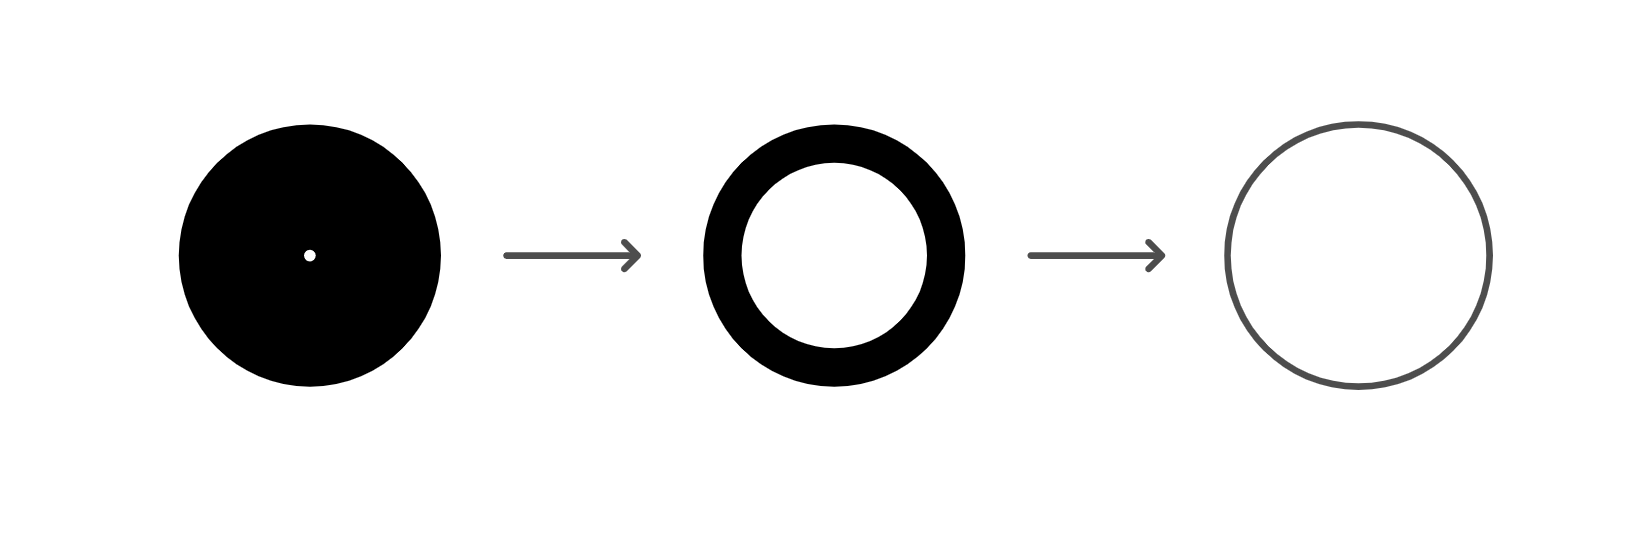
\includegraphics[width=1\linewidth]{def-retract.png}
    \caption{Punktiran disk se deformacijsko retrakira na robno sfero $S^1$}
\end{figure}

Šibko homotopsko ekvivalenco pa opišemo preko homotopskih grup, ki
 jih bomo definirali v nadaljevanju. Prva homotopska grupa se imenuje
  fundamentalna grupa. Je grupa ekvivalenčnih razredov zank v prostoru, 
 tj. poti z enako začetno in končno točko.

Pot v prostoru $X$ je zvezna preslikava $ f\colon  I \rightarrow X$. Poti sta homotopni, če med njima obstaja homotopija rel $\{0,1\}$
\begin{definicija}
    
    \textit{Homotopija poti} v $X$ je družina preslikav $f_t\colon I \rightarrow X, 0\le t \le 1$, taka da
    \begin{itemize}
        \item 
        sta krajišči $f_t(0) = x_0$ in $f_t(1) = x_1$ neodvisni od $t$ in
%t po homotopiji, s po intervalu poti
        \item 
        je prirejena preslikava $F\colon I\times X \rightarrow X$ definirana s $F(t,s) = f_t(s)$ zvezna.
    \end{itemize}
    Za poti $f_1$ in $f_0$, ki sta povezani s homotopijo $f_t$ rečemo, da sta homotopni in označimo $f_1 \simeq f_0$.
\end{definicija}



\begin{trditev}
    Relacija homotopije na poteh s fiksnima krajiščema je ekvivalenčna relacija za vsak topološki prostor.
\end{trditev}

\begin{dokaz}
    Preveriti moramo refleksivnost, simetričnost in tranzitivnost.

    Najprej preverimo refleksivnost. Naj bo $f \colon  I \rightarrow X$ pot v prostoru $X$. Homotopijo definiramo kot $f_t(s)=f(s)$.
    
    Naj velja $f \simeq g$ in naj bo $f_t(s)$ homotopija med $f$ in $g$, 
    torej $f_0=f$ in $f_1=g$. Homotopijo med $g$ in $f$ definiramo kot 
    $g_t(s)=f_{1-t}(s)$. Velja $g_0=f_1=g$ in $g_1=f_0=f$. Ker je 
    $g_t(s)$ kompozitum zveznih preslikav, je zvezna. Sledi, da je 
    relacija homotopije simetrična.
    
    Naj bodo $f, g \text{ in } h$ poti v $X$ in naj velja $f \simeq g$ 
    in $g \simeq h$. Naj bo $f_t(s)$ homotopija med $f$ in $g$ in 
    $g_t(s)$ homotopija med $g$ in $h$. Definirajmo 
    $$h_t(s)=\begin{cases}
        f_{2t}(s), & t \in [0,\frac{1}{2}] \\
        g_{2t-1}(s), & t \in [\frac{1}{2},1]
    \end{cases}
    $$
    Velja $h_0=f_0=f$ in $h_1=g_1=h$. Ker je $h_t(s)$ sestavljena iz dveh zveznih poti, ki se ujemata na preseku, je zvezna, sledi, da je relacija tranzitivna.
\end{dokaz}

Za poljubni poti $f,g \colon  I \rightarrow X$, za kateri velja $f(1) = g(0)$ 
lahko definiramo njun stik $f \sqcdot g$, ki preteče $f$ in $g$ z dvojno 
hitrostjo v enotskem intervalu.
$$ f \sqcdot g(s) \begin{cases}
    f(2s), &s \in [0,\frac{1}{2}] \\
    g(2s-1), & s \in [\frac{1}{2},1]
\end{cases}
$$

Definirajmo še \textit{reparametrizacijo} poti $f$ kot kompozitum $f 
    \varphi$, kjer je $\varphi\colon  I \rightarrow I$ neka zvezna preslikava, za 
    katero velja $\varphi(0)= 0$ in $\varphi(1)=1$. Reparametrizacija poti 
    ohranja homotopski razred, saj sta $f\varphi$ in $f$ povezani preko 
    $f\varphi_t$, pri čemer je $\varphi_t(s)=(1-t)\varphi(s)+ts$. Vidimo, da 
    $\varphi_t(s)$ leži med $\varphi(s)$ in $s$, torej na $I$, zato je 
    $f\varphi_t(s)$ dobro definirana.



    Če se omejimo samo na poti $f\colon I \rightarrow X$ z enako začetno in končno točko $f(0) = f(1) = x_0$, govorimo o zankah. Za $x_0$ rečemo, da je izhodišče.
    Množico vseh homotopskih razredov $[f]$, z izhodiščem $x_0$ označimo s $\pi_1(X,x_0)$.
    

    \begin{izrek}
        $\pi_1(X,x_0)$ opremljena s produktom $[f][g] = [f\sqcdot g]$ je grupa.
    \end{izrek}



\begin{dokaz}
    Najprej preverimo dobro definiranost produkta. Naj velja $[f]=[f']$, preko homotopije $f_t$ in $[g]=[g']$ preko $g_t$. Potem sta $f\sqcdot g$ in $f'\sqcdot g'$ homotopna preko
    $h_t(s) =f_t \sqcdot g_t$. Vidimo, da $h_0=f_0 \sqcdot g_0=f \sqcdot g$ in $h_1=f_1 \sqcdot g_1=f'\sqcdot g'$. Ker je $f_t(1)=g_t(0)$ za vsak t in sta $f_t(s)$ in $g_t(s)$ zvezna, sledi, da je tudi $h_t(s)$ zvezen. Torej velja $[f\sqcdot g]$=$[f'\sqcdot g']$.
    
    Naj bodo $f$, $g$ in $h$ poti v $X$ in naj bo $f(1)=g(0)$ in 
    $g(1)=h(0)$. Potem sta oba stika $(f\sqcdot g) \sqcdot h$ in 
    $f\sqcdot (g \sqcdot h)$ definirana, $(f\sqcdot g) \sqcdot h$ pa je
    reparametrizacija poti $f\sqcdot (g \sqcdot h)$ preko odsekoma linearne 
         funkcije.


Naj bo $f$ pot v $X$ in naj bo $c$ konstantna pot definirana s $c(s)=f(1)$, $f\sqcdot c$ je reparametrizacija $f$ preko 
$$\varphi(s)=\begin{cases}
2s, &s \in [0,\frac{1}{2}] \\
1, & s \in [\frac{1}{2},1],\\
\end{cases}
$$zato velja $f\sqcdot c\simeq f$. Podobno velja tudi  $c\sqcdot f\simeq f$, kjer je $c$ konstantna pot $c(s)=f(0)$. Sklepamo, da je $c(s)=x_0$ dvostranska enota v grupi  $\pi_1(X,x_0)$
     
Inverz poti $f$ definiramo kot $\bar{f}(s)=f(1-s)$. Definirajmo $h_t=f_t\sqcdot \bar{f_t}$, pri čemer je 
$$
f_t(s)=
\begin{cases}
    f(s), &s \in [0,1-t] \\
    f(1-t), & s \in [1-t,1]. \\
\end{cases}
$$
Ker je $h_0=f\sqcdot \bar{f}$ in $h_1=f(0)=c$, sledi, da je $f\sqcdot \bar{f}$ homotopen konstantni poti v $x_0$. Če $f$ zamenjamo z $\bar{f}$, sledi, da $\bar{f}\sqcdot f\simeq c$, zato je $[\bar{f}]$ obojestranski inverz od $[f]$.
\end{dokaz}


Kot že povedano, tej grupi pravimo fundamentalna grupa prostora $X$, z izhodiščem $x_0$. $\pi_1(X,x_0)$ je prva v zaporedju analogno definiranih homotopskih grup $\pi_n(X,x_0)$, pri katerih namesto iz $I$ slikamo iz $n$-dimenzionalne kocke $I^n$.


Naj bo $I^n$ $n$-dimenzionalna kocka. Rob $\partial I^n \text{ od } I^n$ je podprostor točk pri katerih je vsaj ena koordinata enaka $1$ ali $0$. Definirajmo $\pi_n(X,x_0)$, množico homotopskih razredov preslikav $f\colon (I^n,\partial I^n) \rightarrow (X,x_0)$, pri čemer velja $f(\partial I^n) = x_0$.

Za $n\ge 2$ posplošimo stik definiran pri fundamentalni grupi.
$$ f\sqcdot g(s) \begin{cases}
f(2s_1,s_2,\ldots,s_n), & s_1\in [0,\frac{1}{2}] \\
g(2s_1-1,s_2,\ldots,s_n), & s_1 \in [\frac{1}{2},1]
\end{cases}
$$


\begin{izrek}
    $\pi_n(X,x_0)$ opremljena s produktom $[f][g] = [f\sqcdot g]$ je grupa za vsak $n \in \N$.
\end{izrek}

Dokaz te trditve je podoben dokazu za $n=1$, saj je v stik poti vpletena le prva komponenta poti.

\begin{definicija}
    Naj bosta $X$ in $Y$ s potmi povezana topološka prostora.  $X$ in $Y$ sta \textit{šibko homotopsko ekvivalentna}, če obstaja preslikava $f\colon X\rightarrow Y$, ki inducira izomorfizen $\pi_n(X,x_0)\rightarrow \pi_n(Y,f(x_0))$, za vsak $n \in \N$. Preslikavi $f$ rečemo \textit{šibka homotopska ekvivalenca.}
\end{definicija}



Homeomorfni prostori so homotopsko ekvivalentni, homotopsko ekvivalentni prostori so tudi šibko homotopsko ekvivalentni. Dokaz te trditve lahko najdemo v \cite[razdelek 1.1]{hatcher}. Obratno v splošnem ne velja.

%Šibke homotopske ekvivalence imajo lastnost \textit{$2$ od $3$}, kar pomeni, da če sta dve od treh preslikav $f$, $g$ in $fg$ šibki homotopski ekvivalenci, potem je tudi tretja. Dokaz za to trditev lahko najdemo v \cite{hatcher}.

\section{Simplicialni kompleksi}\label{sec:simpleks}


\begin{definicija}
    \textit{Simplicialni kompleks $K$} je podan z množico \textit{oglišč} $V=V_K$ in množico $S=S_K$ končnih nepraznih podmnožic $V$, imenovanih \textit{simpleksi}, ki ustrezajo pogoju, da je vsaka podmnožica simpleksa tudi simpleks. Pišemo $\sigma \in K$ in $v \in K$, če je $\sigma \in S_K$ ter $v \in V_K$. 
\end{definicija}

\textit{Dimenzija} simpleksa $\sigma$ je enaka ena manj od števila njegovih oglišč. Simpleksu dimenzije $n$ rečemo $n-$simpleks. Dimenzija simplicialnega kompleksa $K$ je enaka maksimumu dimenzij njegovih simpleksov, $n$-dimenzionalnemu simplicialnemu kompleksu rečemo tudi \textit{n-kompleks}. Omejili se bomo samo na končne komplekse, torej $n \in \N$.


\textit{Podkompleks} $L\subseteq K$ simplicialnega kompleksa $K$ je simplicialni kompleks, za katerega velja $V_L\subseteq V_K$ in $S_L\subseteq S_K$.


 Naj bo $\sigma = \{v_0,v_1,\ldots,v_n\}$ $n$-simpleks. Zaprt
 simpleks $\bar{\sigma}$ je množica formalnih konveksnih kombinacij $\sum\limits_{i=0}^{n}\alpha_i v_i$
 pri čemer je $\alpha_i \ge 0$ za vsak $0\le i \le n$ in $\sum\limits_{i=0}^{n}\alpha_i = 1$. Zaprt simpleks je metričen prostor z metriko
 
 \begin{equation}
     d\biggl(\sum\limits_{i=0}^{n}\alpha_i v_i,\sum\limits_{i=0}^{n}\beta_i v_i \biggr) = \sqrt{\sum\limits_{i=0}^{n}(\alpha_i - \beta_i)^2}.
     \label{eq:metrika}    
 \end{equation}
 Če so $v_i$ linearno neodvisne točke v $\R^m$ za nek $m\geq n$, potem je $\bar{\sigma}$ homeomorfen prostoru 
 $\Bigl\{ \sum\limits_{i=0}^{n}\alpha_i v_i, | \sum\limits_{i=0}^{n}\alpha_i = 1 \text{ in } \alpha_i \ge 0 \Bigr\}\subseteq \R^m$. To pomeni, da lahko vsak zaprt simpleks predstavimo kot podprostor $\R^m$ z evklidsko topologijo.


 %opomba??????
 \textit{Geometrijska realizacija} $|K|$ simplicialnega kompleksa $K$ je 
 množica formalnih konveksnih kombinacij $\underset{v \in V_K}{\Sigma}\alpha_v v$, takih da je $\{v | \alpha_v > 0\}$ simpleks v $K$ in 
 $\Sigma_{v\in V_K}\alpha_v=1$. Rečemo, da $|K|$ realizira $K$. Za točko $\alpha=\underset{v \in V_K}{\Sigma}\alpha_v v \in |K|$ označimo $\supp(\alpha)=\{v | \alpha_v > 0\}$, 
 tej množici pravimo nosilec od $\alpha$. Topologijo na $|K|$ definiramo na naslednji način. $U \subseteq |K|$ je odprta, natanko tedaj, ko je $U \cap 
 \si$ odprta v $\si$, za vsak $\sigma \in K$. Kot prej, če so $v\in K$ linearno neodvisne točke v $\R^m$ za nek $m\geq |V_K|$, potem je 
 $|K|$ homeomorfen prostoru 
 $$\bigl\{\Sigma_{v\in K}\alpha_v v | \Sigma_{v\in K} \alpha_v = 1 \text{, } \alpha_i
 \ge 0 \text{ in } \{v | \alpha_v > 0\} \text{ je simpleks v $K$}\bigr\} \subseteq \R^m.$$ To pomeni, da lahko vsak simplicialni
 kompleks predstavimo kot podprostor v $\R^{|V_K|}$ z evklidsko topologijo.
 Če $L\subseteq K$, potem je $|L|\subseteq |K|$ zaprta podmnožica.
 
 \begin{opomba}
     Če je $K$ $n-$kompleks, potem se ga da realizirati v $\R^{2n+1}$. To pomeni, da obstaja podprostor v
     $\R^{2n+1}$, ki je homeomorfen $|K|$. Vsak enostaven graf je geometrijska realizacija $1-$kompleksa, zato ga 
     lahko realiziramo v $\R^{2\cdot 1 +1}=\R^{3}$, kar je pa znano dejstvo iz teorije grafov.
 \end{opomba}
 
 
 \textit{Polieder} je geometrijska realizacija simplicialnega kompleksa $|K|$. \textit{Triangulacija} poliedra $X$ je simplicialni kompleks, katerega geometrijska realizacija je homeomorfna $X$.
 
Preslikava $f$ iz $|K|$ v nek topološki prostor $X$ je zvezna, natanko tedaj, ko je $f|_{\bar{\sigma}}\colon  \bar{\sigma} \rightarrow X$ zvezna za vsak $\sigma\in K$.
Saj je $U \subseteq |K|$ odprta, natanko tedaj, ko je $U \cap 
\si$ odprta v $\si$, za vsak $\sigma \in K$.
Tudi $H\colon |K|\times I \rightarrow X$ je zvezna, natanko tedaj, ko je zvezna $H|_{\si\times I}\colon \si\times I \rightarrow X$, za vsak $\sigma\in K$.
 
 
 \textit{Simplicialna preslikava} $\varphi \colon K \rightarrow L$, med 
 simplicialnima kompleksoma $K$ in $L$, je preslikava med 
 oglišči, $V_K \rightarrow V_L$, ki slika simplekse v 
 simplekse. Preslikava $\varphi$ inducira zvezno preslikavo med 
 kompleksoma $|\varphi| \colon |K| \rightarrow |L|$, kot $|\varphi|\colon 
 \underset{v \in K}{\Sigma}\alpha_v v \mapsto
 \underset{v \in K}{\Sigma}\alpha_v \varphi(v)$.
 
     
 %\textit{Baricentrična subdivizija} simplicialnega kompleksa 
 %$K$ je simplicialni kompleks $K'$, čigar oglišča so 
 %simpleksi $\sigma \in K$, simpleksi v $K'$ so pa verige 
 %simpleksov v $K$, urejenih z inkluzijo. Torej $\sigma' \in K'$, če $\sigma' = \{\sigma_0, \sigma_1, \cdots ,\sigma_n\}$ in $\sigma_0\subsetneq \sigma_1\subsetneq \cdots \subsetneq\sigma_n$. \textit{Težišče} simpleksa $\sigma \in K$ je točka $b(\sigma)=\underset{v\in \sigma}{\Sigma} \frac{v}{\#\sigma}$.
 
 %Definirajmo linearno preslikavo $S_K\colon  |K'| \rightarrow |K|$, s predpisom $S_K(\sigma) = b(\sigma)$. Linearnost pomeni, da velja $S_K(\underset{\sigma\in \sigma'}{\Sigma} a_\sigma \sigma) =  \underset{\sigma\in \sigma'}{\Sigma} a_\sigma S_K(\sigma).$
 
 %\begin{primer}
 %Naj bo $K=\sigma=\{\{a\},\{b\},\{c\},\{a,b\},\{a,c\},\{b,c\},\{a,b,c\}\}$ 
 
 %$3-$simpleks.
 %\begin{figure}[h]
 %    \centering
 %    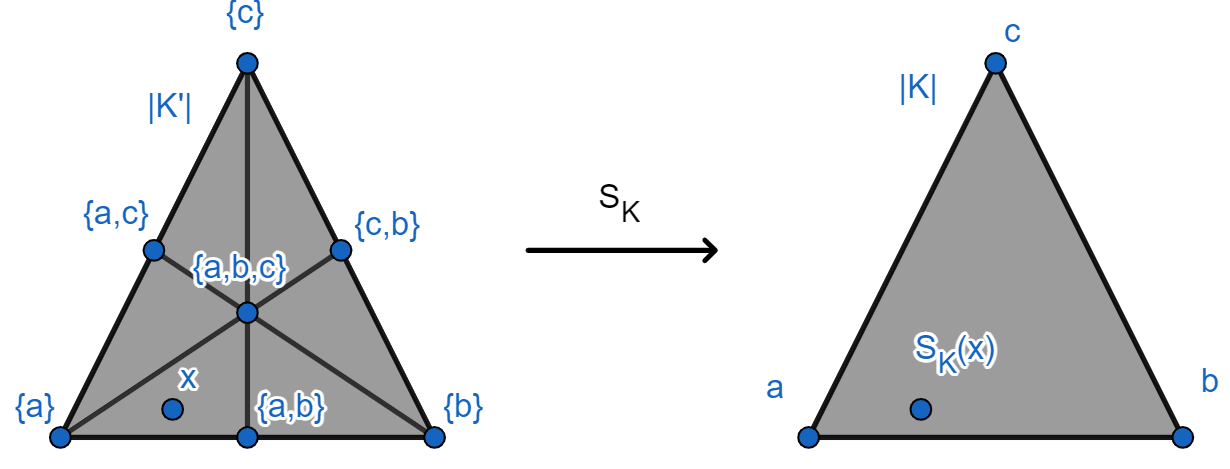
\includegraphics[width=0.7\linewidth]{sk.png}
 %\end{figure}
 %Poglejmo si preslikavo $S_K\colon  |K'| \rightarrow |K|$. Naj bo $x$ tako kot na sliki. %Zaradi preglednosti označimo
 
 %Potem je 
 %$K'_x\colon =\supp(x)=\{\{a\},\{a,b\},\{a,b,c\}\}$ in $x= \underset{\sigma\in K'_x}{\Sigma} \alpha_{i_\sigma} \sigma$. Zato
 
 %\begin{align*}
% S_K(x)&=S_K(\underset{\sigma\in K'_x}{\Sigma} \alpha_{i_{\sigma}} 
 % \sigma) =  \underset{\sigma\in K'_x}{\Sigma} \alpha_{i_{\sigma}} 
 %S_K(\sigma)\\
 %&=\alpha_1S_K(\{a\})+\alpha_2S_K(\{a,b\})+\alpha_3S_K(\{a,b,c\}) \\ 
 %&=\alpha_1a+\alpha_2\frac{a+b}{2}+\alpha_3\frac{a+b+c}{3}.
 %\end{align*}
 %Preslikava $S_K$ je očitno homeomorfizem.
 
 
 
 %\end{primer}


 \begin{trditev}
    Naj bosta $K$ in $L$ simplicialna kompleksa in naj bosta $f,g\colon |K|\rightarrow |L|$ taki zvezni preslikavi, da za vsak $\alpha\in |K|$ obstaja $\sigma \in L$, da $f(\alpha),g(\alpha) \in \overline{\sigma}.$ Potem sta $f$ in $g$ homotopni.
    \label{tr:shom}
\end{trditev}

\begin{dokaz}
    Preslikava $H\colon |K|\times I\rightarrow |L|$, definirana kot $H(x,t)=tg(x) + (1-t)f(x)$ je dobro definirana, ker $f(x)$ in $g(x)$ ležita v istem zaprtem simpleksu. $H$ je zvezna, natanko tedaj, ko je zvezna zožitev $H|_{\overline{\sigma}\times I}\colon \overline{\sigma}\times I \rightarrow |L|$, za vsak $\sigma \in K$. Zožitev pa je zvezna, saj je kompozitum dveh zveznih preslikav. Torej zveznost $H$ sledi iz zveznosti $f$ in $g$.
%\begin{align*}
 %   d(H(x,t)&,H(y,s)\leq d(tg(x)+(1-t)f(x),sg(x)+(1-s)f(x)) \\
%&+d(sg(x)+(1-s)f(x),sg(y)+(1-s)f(y))\\
%&\leq 2|t-s|+d(f(x),f(y))+d(g(x),g(y)).
%\end{align*}

\end{dokaz}

\begin{definicija}
    Simplicialni preslikavi $\varphi, \psi\colon K\rightarrow L$ sta \textit{bližnji}, če je za vsak $\sigma \in K$, $\varphi(\sigma)\cup \psi(\sigma)$ simpleks v $L$.
\end{definicija}

Če sta $\varphi$ in $\psi$ bližnji, potem $|\varphi|$ in $|\psi|$ zadostita predpodstavkam v trditvi \ref{tr:shom}, saj če $x\in \overline{\sigma}$, potem $|\varphi|(x)$ in $|\psi|(x)$ ležita v $\overline{\varphi(\sigma)\cup\psi(\sigma)}$. Takoj sledi naslednja posledica.

\begin{posledica}
    Če sta $\varphi$ in $\psi$ bližnji, sta $|\varphi|$ in $|\psi|$ homotopni.
\end{posledica}

\textit{Simplicialni stožec z vrhom $v$} je simplicialni kompleks $K$ z ogliščem $v$, za katerega velja, da je $\sigma \cup \{v\} \in K$, za vsak simpleks $\sigma\in K$.

\begin{posledica}
    Če je $K$ simplicialni stožec, potem je $|K|$ kontraktibilen.
    \label{pos:kontr}
\end{posledica}

\begin{dokaz}
    Naj bo $v$ vrh od $|K|$. Po definiciji simplicialnega stožca, je simplicialna preslikava, ki slika vsako oglišče v $v$, kontiguentna identiteti. Zato je identiteta v $|K|$ homotopna konstantni preslikavi.
\end{dokaz}

\subsection{Poti v simplicialnem kompleksu}

\textit{Rob} simplicialnega kompleksa $K$ je urejeni par $e=(v_0,v_1)$, tak da je $\{v_0,v_1\}$ simpleks v $K$. Oglišču $v_0$ rečemo \textit{začetek} $e$ in označimo 
$v_0=\mathfrak{o}(e)$, oglišču $v_1$ pa \textit{konec} $e$, 
označimo $\mathfrak{e}(e)=v_1$. \textit{Lomljenka} dolžine $n$ je stik $n+1$ robov v $K$ $e_0e_1 \cdots e_{n}$, za katerega velja, da je $\mathfrak{e}(e_i)=\mathfrak{o}(e_{i+1})$, za vsak $0\leq i \leq n-1$.
Lomljenka je sklenjena, če $\mathfrak{o}(e_0)=\mathfrak{e}(e_n)$. Oglišču $v_0$ rečemo izhodišče. Če sta $\xi =e_0e_1 \cdots e_n$ in $\xi'=e'_0e'_1 \cdots e'_{m}$ in velja $\mathfrak{e}(e_n)=\mathfrak{o}(e'_0)$ definiramo stik lomljenk $\xi\xi'$ kot $e_0e_1 \cdots e_{n}e'_0e'_1 \cdots e'_{m}$.

Lomljenki $\cdots(v_i,v_{i+1})(v_{i+1},v_{i+2})\cdots$ in $\cdots(v_i,v_{i+2})\cdots$ sta \textit{elementarno ekvivalentni}, če je $\{v_i,v_{i+1},v_{i+2}\}$ simpleks v $K$. Lomljenki $\xi_0$ in $\xi_n$ sta ekvivalentni, če obstaja zaporedje lomljenk $\xi_0,\xi_1,\cdots,\xi_n$, pri katerem sta $\xi_i$ in $\xi_{i+1}$ elementarno ekvivalentni za vsak $0\leq i < n$


\begin{figure}[h]
    \centering
    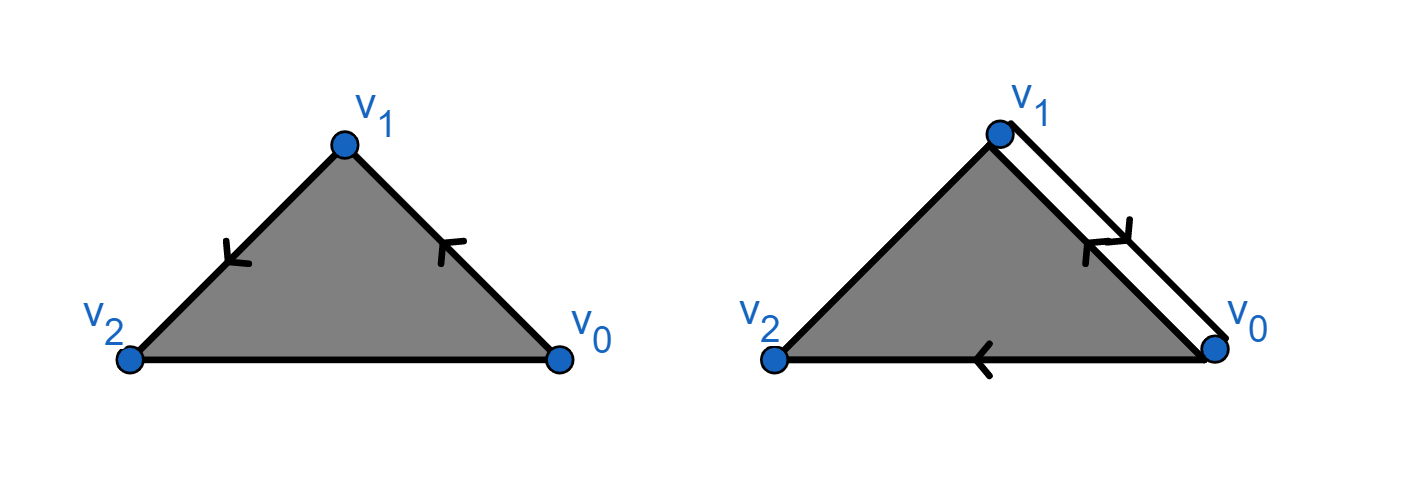
\includegraphics[width=0.9\linewidth]{lomljenki2.png}
    \caption{lomljenki $(v_0,v_1)(v_1,v_2)$ in $(v_0,v_1)(v_1,v_0)(v_0,v_2)$ sta ekvivalentni.}
\end{figure}

    Naj bo $K$ simplicialni kompleks in $v_0$ oglišče v $K$. Z $E(K,v_0)$ označimo množico ekvivalenčnih razredov sklenjenih lomljenk z izhodiščem v $v_0$. Ekvivalenčni razred sklenjene lomljenke $\xi$ označimo z $[\xi]$.

    \begin{trditev}
        Množica $E(K,v_0)$ z množenjem, ki ga inducira stik lomljenk, tvori grupo.
    \end{trditev}
\begin{dokaz}
    Asociativnost je očitna. Naj bo $[\xi_0]=[\xi_n]$ in $[\eta_0]=[\eta_n]$. Naj bosta $\xi_0,\xi_1,\cdots \xi_n$ in $\eta_0,\eta_1,\cdots \eta_n$ zaporedji lomljenk, v katerih sta sosednji lomeljenki elementarno ekvivalentni. Potem je $\xi_0\eta_0,\xi_1\eta_0,\cdots \xi_n\eta_0,\xi_n\eta_1,\cdots, \xi_n\eta_n$ zaporedje lomljenk v katerem sta sosednji preprosto ekvivalentni in zato $[\xi_0\eta_0]=[\xi_n\eta_n]$.
        Enota je ekvivalenčni razred poti $(v_0,v_0)$. Inverz 
    od $e_0e_1 \cdots e_{n-1}e_n$ je $e^{-1}_n e^{-1}_{n-1} \cdots e^{-1}_1$ $e^{-1}_0$, kjer $(v_i,v_{i+1})^{-1}=(v_{i+1},v_i)$.
\end{dokaz}

\begin{izrek}
    $E(K,v_0)$ je izomorfna $\pi_1(|K|,v_0)$
    \label{iz:grupa lomljenk}
\end{izrek}

Dokaz lahko najdemo v \cite[razdelek 3.6]{spanier}

\section{Končni topološki prostori in delno urejene množice}
\label{sec:delne}

\textit{Končni topološki prostor} je topološki prostor s končno mnogo točkami, 
\textit{šibko urejena} množica je množica s tranzitivno in z refleksivno relacijo. Če je relacija še antisimetrična, dobimo \textit{delno} ureditev.
\\ \indent Naj bo $X$ končni topološki prostor in $x \in X$. Družina vseh odprtih množic, ki vsebujejo $x$ je končna, zato je njen presek $U_x$ najmanjša odprta množica, ki vsebuje $x$.
    Točke uredimo s pravilom $ x\le y \text{, če } U_x \subseteq  U_y$. S tem dobimo šibko ureditev. 
    Antisimetričnost po definiciji sovpada z lastnostjo $T_0$, zato, relacija postane delna ureditev,
     natanko takrat, ko je topologija $T_0$.
    \\ \indent Obratno, naj bo končna $X$ šibko urejena množica. Na njej lahko definiramo topologijo z bazo $\{y \in X | y\le x\}_{x \in X}$. Če je
$y \le x$, je $y$ vsebovan v vsaki bazni množici, ki vsebuje $x$, torej je $y \in U_x$. Po drugi strani, če je $y\in
U_x$, potem je $y \in \{y \in X | y \le x\}$, torej velja, da je $y \le x$ natanko tedaj, ko je $y \in U_x$. S tem dobimo zvezo med končnimi prostori in končnimi šibkimi ureditvami. %%opomba????

Omejili se bomo na končne $T_0$ prostore in na končne delne ureditve. V nadaljevanju ne bomo več razlikovali med delnimi ureditvami in $T_0$ prostori, kar pomeni, da za prostor $X$ in $x,y\in X$, $x\leq y$ pomeni ureditev v prirejeni delni urejenosti oziroma da velja $x\in U_y$. 

Delno urejene množice pogosto predstavljamo s Hassejevimi diagrami, zato bomo tudi končne $T_0$ prostore predstavljali na tak način.

\begin{definicija}
    \textit{Hassejev diagram} delno urejene množice $X$ je usmerjen graf, katerega oglišča so točke, povezave pa so urejeni pari $(x,y)$, taki, da je  $x<y$ in ne obstaja tak $z$, da bi veljalo $x<z<y$.
\end{definicija}

Povezave $(x,y)$ ne rišemo s puščico iz $x$ v $y$, ampak bomo $x$ in $y$ povezali z ravno črto in $y$ pisali nad $x$. Če je $(x,y)$ povezava v Hassejevem diagramu končne delno urejene množice, rečemo, da $y$ \textit{pokrije} $x$ in pišemo $x\prec y$.

\begin{primer}
    Naj bo $X=\{a,b,c,d\}$ končen prostor, s topologijo 
    $\tau=\{\emptyset,X,\{b,d\},$ $\{c\},\{d\},\{b,c,d\},
    \{c,d\}\}$. Topologija je $T_0$, zato je $X$ tudi delno 
    urejena množica.
\begin{figure}[h!]
    \centering
    \begin{minipage}{0.5\textwidth}
        \centering
        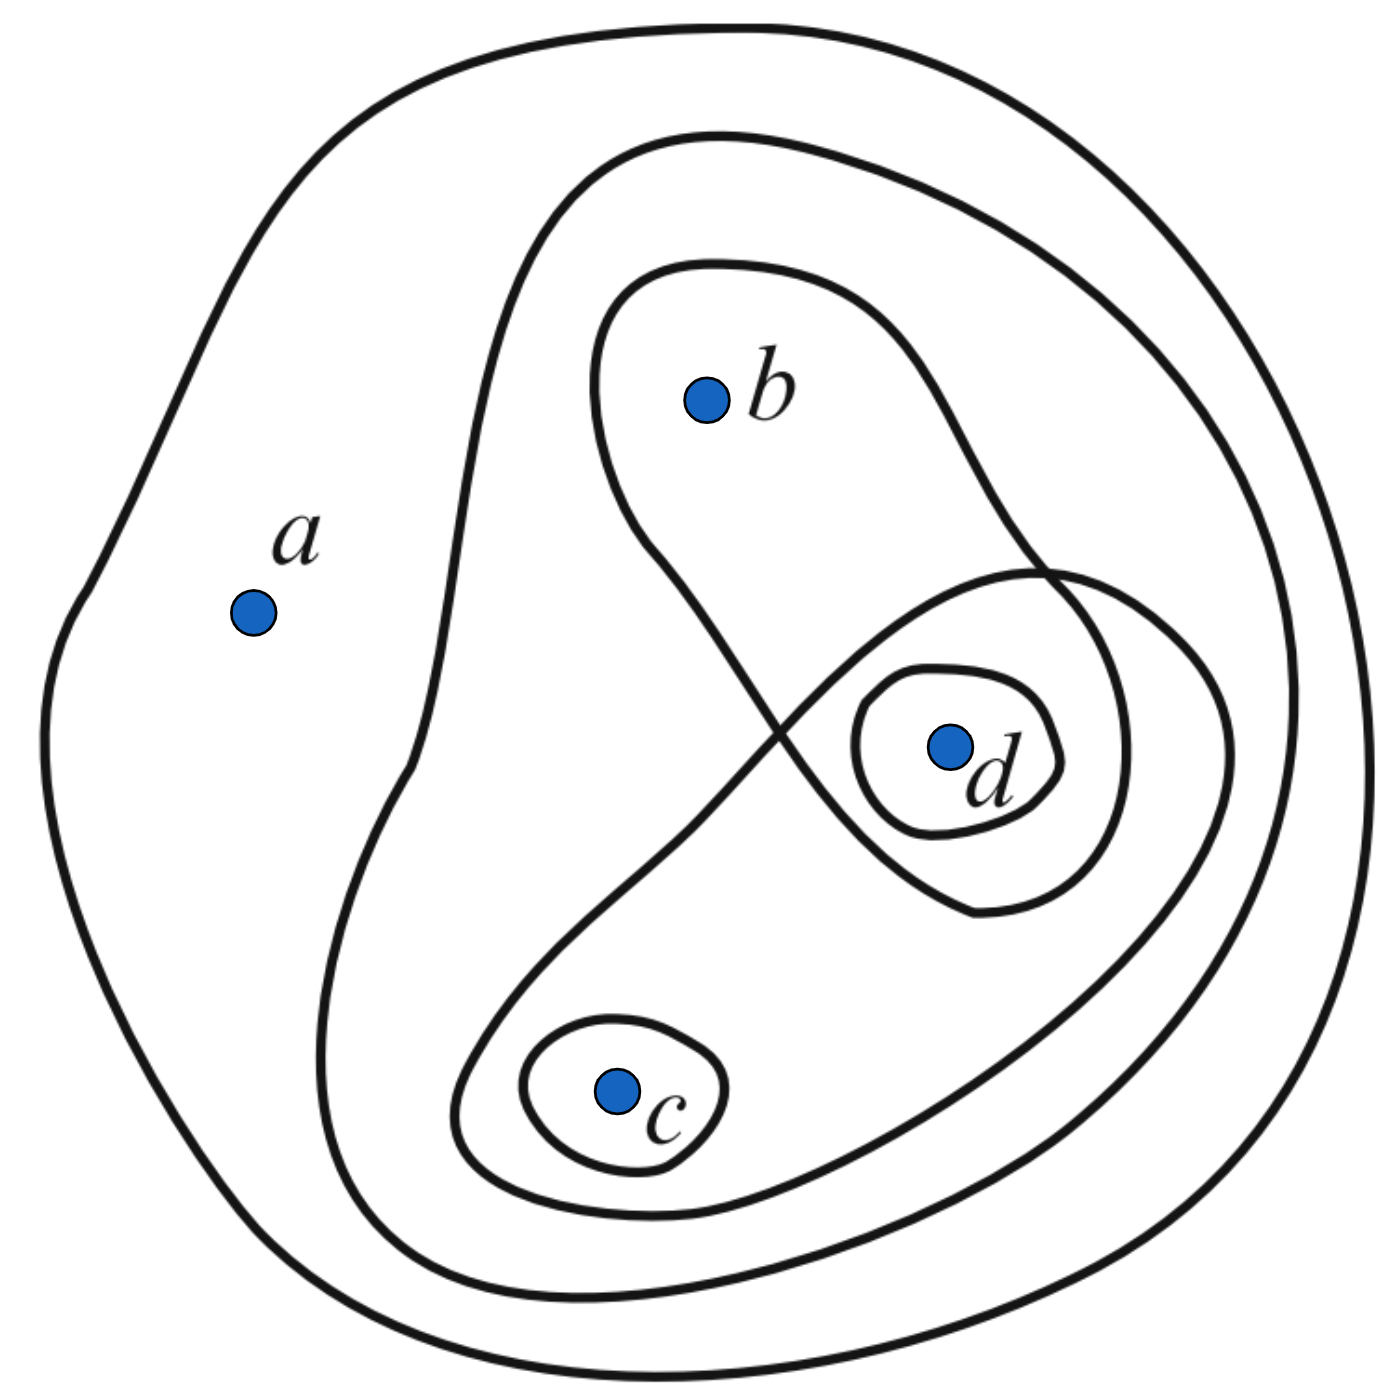
\includegraphics[width=0.6\linewidth]{open.png}
    \end{minipage}%
    \begin{minipage}{0.5\textwidth}
        \centering
        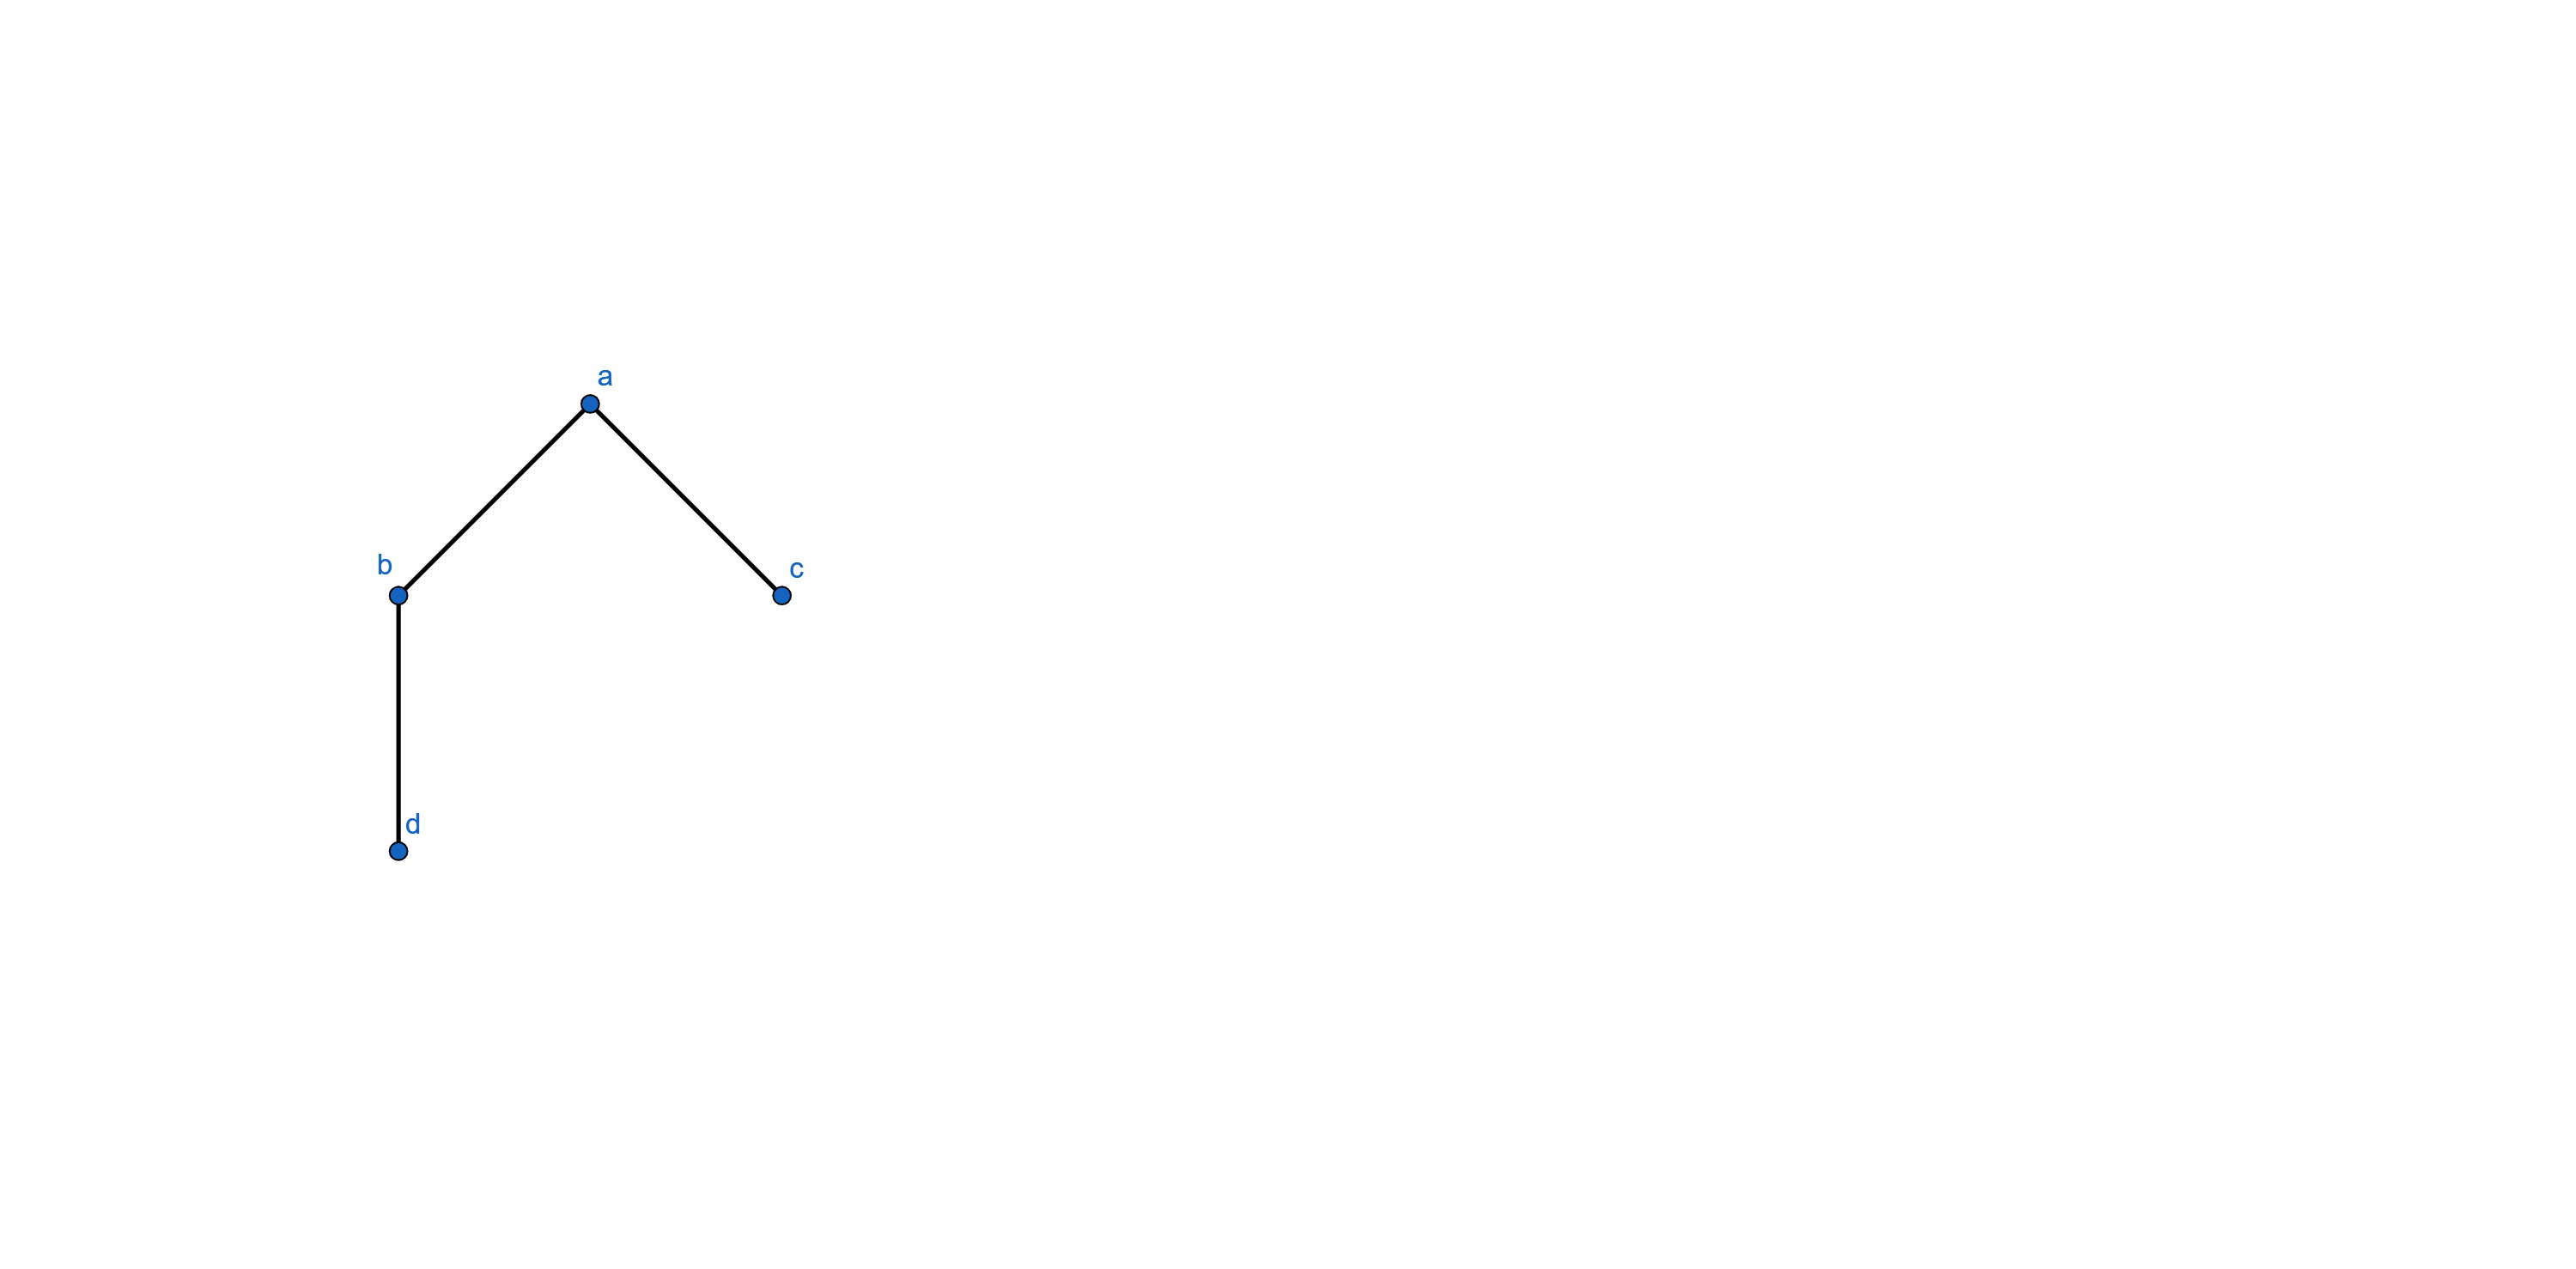
\includegraphics[width=2.5\linewidth]{hasse.png}
    \end{minipage}
    \caption{Odprte množice v $X$ in prirejen Hassejev diagram.}
\end{figure}


\end{primer}

\begin{definicija}
    Element $x\in X$ je \textit{maksimalni element} delno urejene množice $X$, če $\forall y \in X, y\geq x \Rightarrow y = x$,
    $x$ je \textit{maksimum} v $X$, če $\forall y \in X, x\geq y$.
\end{definicija}

Končna delno urejena množica ima maksimum, natanko tedaj, ko ima enoličen maksimalni element. \textit{Minimalni element} in \textit{minimum} definiramo analogno.

Elementa $x$ in $y$ sta \textit{primerljiva}, če je $x\leq y$ ali $y\leq x$. \textit{Veriga} v $X$ je podmožica $S\subseteq X$, v kateri je vsak par elementov primerljiv, \textit{antiveriga} v $X$ je podmožica $S\subseteq X$, v kateri ni noben par elementov primerljiv. 

Odprtim množicam v $X$ ustrezajo \textit{navzdol zaprte množice}, zaprtim pa \textit{navzgor zaprte množice}. Podmnožica $U$
 delno urejene množice $X$ je navzdol zaprta, če $\forall x\in X,$ iz $y\leq x$, sledi da $y\in U$. Navzgor zaprte množice definiramo analogno.
Z $F_x$ označimo zaprtje množice $\{x\}$. $F_x:=\{y\in X; y\geq x\}$. Vidimo, da $y\in F_x \Leftrightarrow x\in U_y$.

Tudi morfizmi delno urejenih množic in morfizmi končnih topoloških prostorov sovpadajo.
  Morfizem delno urejene množice je preslikava, ki ohranja ureditev, oziroma monotona preslikava, torej $f\colon  X\rightarrow Y$, 
  za katero iz $x\leq x'$ sledi $f(x)\leq f(x')$ za vsaka $x,x'\in X$. Morfizmi topoloških prostorov so pa zvezne preslikave.

\begin{trditev}
Preslikava $f\colon X\rightarrow Y$ med končnima prostoroma je zvezna, natanko tedaj, ko je monotona.
\end{trditev}
%opomba??????

%\begin{dokaz}
 %   Naj bo preslikava $f$ zvezna in naj $x\leq x'$ za $x, x' \in X$. Zaradi zveznosti je $f^{-1}(U_{f(x')})$ odprta. Ker velja $f(x')\in U_{f(x')}$, sledi, da $x'\in f^{-1}(U_{f(x')})$, ker je to navzdol zaprta množica, je tudi $x\in f^{-1}(U_{f(x')})$, na enakosti uporabimo $f$ in dobimo $f(x)\in U_{f(x')}$, torej $f(x)\leq f(x')$ in je $f$ monotona.
%
 %   Naj bo zdaj $f$ monotona preslikava. Pokažimo, da je $f^{-1}(U_y)$ navzdol zaprta množica za vsako bazno množico $U_y$. Naj bo $x\leq x'$ in $x'\in f^{-1}(U_y)$, torej $f(x') \in U_y$, ker je f monotona in je $U_y$ navzdol zaprta, sledi da $f(x)\in U_y$, zato je $x\in f^{-1}(U_y)$, torej je $f^{-1}(U_y)$ navzdol zaprta, torej odprta.
%\end{dokaz}

\begin{dokaz}
    Naj bo $f$ zvezna in naj $x\leq y$ za $x, y \in X$. Če z $F_x$ označimo zaprtje množice $\{x\}$, je potem $F_y \subseteq F_x$. Iz zveznosti pa sledi $f(F_x)\subseteq F_{f(x)}$. Velja $f(F_y) \subseteq f(F_x) \subseteq F_{f(x)}$. Recimo, da preslikava $f$ ni monotona in velja $f(x) > f(y)$. Potem velja $f(y) \notin F_{f(x)}$, ampak iz tega sledi $f(y) \notin f(F_y)$, kar je pa protislovje, zato je $f$ monotona.


    Naj bo zdaj $f$ monotona preslikava in $A\subseteq X$ poljubna množica. Dokažimo da velja $f(\overline{A}) \subseteq \overline{f(A)}$. Naj bo $y\in f(\overline{A})$, potem $y=f(x)$ za nek $x\geq a$ in $a\in A$. Ker je $f$ monotona, velja $f(x) \geq f(a)$. Torej $y \geq f(a)$ in zato $y\in \overline{f(A)}$. Torej je $f$ zvezna.
\end{dokaz}


\begin{lema}
    Za vsaki primerljivi točki $x,y\in X$ v končnem prostoru $X$ obstaja pot od $x$ do $y$, tj. preslikava $\alpha\colon  I \rightarrow X$, za katero velja $\alpha(0)=x$ in $\alpha(1)=y$.
\label{lem:pot}
\end{lema}
\begin{dokaz}
    Naj bo $x \leq y$. Definirajmo $\alpha\colon I\rightarrow X$, z $\alpha([0,1))=x$ in $\alpha(1)=y$ in naj bo $U \subseteq X$ odprta. Če $U$ vsebuje $y$, mora vsebovati tudi $x$, 
    zato je praslika od $U$ ali $\emptyset$ ali $[0,1)$ ali pa $I$, ki so pa vse odprte v $I$, zato je $\alpha$ pot od $x$ do $y$.

    Če je pa $x \geq y$, definiramo $\alpha\colon I\rightarrow X$, z $\alpha((0,1])=y$ in $\alpha(0)=x$. Za odprto množico $U\subseteq X$ so možne praslike $\emptyset$, $(0,1]$ in $I$, ki so vse odprte v $I$.
\end{dokaz}
Ta lema nam pove, da v končnih prostorih obstajajo netrivialne poti, zato v splošnem fundamentalna grupa končnega prostora ni trivialna.

Naj bosta $X$ in $Y$ delni ureditvi. Z $Y^X$ označimo končno množico zveznih preslikav iz $X$ v $Y$ in jo opremimo z ureditvijo po točkah in sicer $f\leq g$, če velja $f(x) \leq g(x), \forall x\in X$. S tem dobimo na $Y^X$ delno ureditev in topologijo, ki je enaka kompaktno-odprti topologiji.  %opomba???

\textit{Ograja} v $X$ je zaporedje $x_0,x_1, \cdots ,x_n$ točk v $X$, taka, da sta vsaki zaporedni točki primerljivi. $X$ je \textit{urejenostno povezan}, če za vsaki točki $x,y\in X$ obstaja ograja, ki se začne z $x$ in konča z $y$.
\begin{lema}
    Naj bo $X$ končen $T_0$ prostor. Naslednje trditve so ekvivalentne:

    \begin{itemize}
        \item $X$ je povezan prostor.
        \item $X$ je urejenostno povezana delna ureditev.
        \item $X$ je povezan s potmi.
    \end{itemize}
    \label{lem:povezanost}
\end{lema}


\begin{dokaz}
    Če je $X$ urejenostno povezan, potem je po lemi \ref{lem:pot}, povezan tudi s potmi.
    Dokazati je treba le še da urejenostna povezanost sledi iz povezanosti. Naj bo torej $X$ povezan, $x\in X$ in $A=\{y\in X| \text{ obstaja ograja med $x$ in $y$}\}$. Če 
    je $z\leq x$, potem je tudi $z\in A$, zato je $A$ navzdol zaprta. Analogno pokažemo, da je $A$ navzgor zaprta. Ker je $X$ povezan, sledi, da $A=X$, zato je $X$ urejenostno povezan.
\end{dokaz}

\begin{trditev}
    Naj bosta $f,g\colon  X\rightarrow Y$ preslikavi med končnima prostoroma in $A\subseteq X$, potem je $f\simeq g$ rel $A$, natanko tedaj, ko obstaja ograja $f=f_0\leq f_1\geq  \cdots  f_n=g$, taka da $f_i|_A=f|_A$. Če je $A=\emptyset$, dobimo navadno homotopijo med $f$ in $g$
    \label{iz:ograje}
\end{trditev}

\begin{dokaz}
    Obstoj homotopije $H\colon f\simeq g$ rel $A$ je ekvivalenten obstoju take poti $\alpha\colon  I \rightarrow Y^X$, da velja $\alpha(t)|_A=f|_A$, kar je ekvivalentno obstoju poti 
    $\alpha\colon  I \rightarrow M$, kjer je $M\subseteq Y^X$ množica, ki vsebuje preslikave, ki na $A$ sovpadajo z $f$. Po lemi \ref{lem:povezanost} to pomeni, da obstaja ograja 
    med $f$ in $g$ v $M$.
\end{dokaz}


\begin{trditev}
    Naj bo $X$ končen prostor in naj bo $X_0$ kvocient $X/_\sim$, pri čemer $x\sim y \Leftrightarrow x\le y$ in $y\le x$. Potem je $X_0\in T_0$, kvocientna projekcija $q\colon X\rightarrow X_0$ pa je homotopska ekvivalenca.
\end{trditev}

\begin{dokaz}%opomoba??? očitno
    Naj bo $i\colon X_0\rightarrow X$ preslikava, za katero velja $qi=1_{X_0}$, $i$ je monotona, zato je zvezna. Ker velja tudi $iq \leq 1_X$, je $i$ homotopski inverz od $q$.

    Naj bosta $x,y\in X$ taka, da $q(x)\leq q(y)$. Po definiciji je $iq \leq 1_X$ in $iq \geq 1_X$, zato je $x \leq iq(x) \leq iq(y) \leq y$. Če velja še $q(y)\leq q(x)$, potem je tudi $y\leq x$, ampak potem je $q(x)=q(y)$, zato je šibka ureditev na $X_0$ antisimetrična, torej je $X_0\in T_0$.
    
    Ker je $iq\leq 1_X$ ter $iq$ in $1_X$ sovpadata na $i(X_0)$ je po trditvi \ref{iz:ograje} 
    $iq \simeq 1_{X_0}$ rel $X_0$, zato je $X_0$ krepki deformacijski retrakt od $X$.
\end{dokaz}
    
Trditev nam pove, da je vsak končen topološki prostor homotopsko ekvivalenten končnemu prostoru, ki ima lastnost $T_0$. Zato smo se v poglavju lahko omejii na $T_0$ prostore in prirejene delne ureditve.

\begin{definicija}
    Točka $x \in X$ je \textit{navzdol odvečna}, če ima $\widehat{U}_x:=\{y\in X | y < x\}$ maksimum in \textit{navzgor odvečna}, če ima $\widehat{F}_x:=\{y\in X | y > x\}$ minimum. 
    Točka je odvečna, če je eno ali drugo.
\end{definicija}

Navzgor odvečne točke v Hassejevem diagramu so tiste, ki imajo 
izhodno stopnjo enako ena, navzdol odvečne, pa tiste, ki imajo vhodno stopnjo enako ena.
\begin{trditev}
Naj bo $X$ $T_0$ prostor in $x\in X$ odvečna točka, potem je $X\backslash \{x\}$ krepki deformacijski retrakt od $X$.
\end{trditev}

\begin{dokaz}
Recimo, da je $x$ navzdol odvečna točka, in naj bo $y$ 
maksimum v $\widehat{U}_x$. Definirajmo retrakcijo $r\colon X\rightarrow 
X\backslash \{x\}$ z $r(x')=x'$ za $x'\neq x$ in $r(x)=y$ in z $i\colon X\backslash\{x\} 
\rightarrow X$ označimo inkluzijo. Ker je $r$ monotona, saj je $x\leq y$, je tudi zvezna. Poleg tega je $ir\leq 1_X$, zato iz trditve \ref{iz:ograje} sledi $ir \simeq 1_x$ rel 
$X\backslash\{x\}$. Za navzgor odvečne točke, je 
dokaz analogen.
\end{dokaz}

\begin{definicija}
    $T_0$ prostor je \textit{minimalen}, če nima odvečnih točk. Krepki deformacijski retrakt prostora $X$, ki je minimalen prostor imenujemo \textit{jedro} končnega prostora $X$.
\end{definicija}

Končnemu prostoru $X$ postopoma odstranjujemo odvečne točke in s tem v vsakem koraku dobimo prostor, ki je homotopsko ekvivalenten prostoru $X$, zato je jedro krepki deformacijski retrakt začetnega prostora, torej mu je homotopsko ekvivalenten. Seveda so tudi vsa jedra istega prostora homotopsko ekvivalentna.

\begin{izrek}
    Naj bo $X$ končen minimalen prostor. Preslikava $f\colon X\rightarrow X$ je homotopna identiteti, natanko tedaj, ko je $f=1_X$.
    \label{iz:identiteta}
\end{izrek}

\begin{dokaz}
    Po trditvi \ref{iz:ograje} lahko predpostavimo, da je
    $f\leq 1_X$ ali $f\geq 1_X$. %zakaj je to res???
    Pa recimo, da velja $f\leq 1_X$. 
    Za $x\in X$ dokažemo $f(x)=x$ z indukcijo na 
    število elementov v $U_x$. Če $U_x=\{x\}$, potem je 
    $f(x)=x$, saj je $f$ monotona, če $U_x\neq\{x\}$, potem 
    je po indukcijski predpostavki 
    $f|_{\widehat{U}_x}=1_{\widehat{U}_x}$. Če $f(x)=x$, potem je 
    $f(x)\in \widehat{U}_x$ in $\forall y < x, y=f(y)\leq 
    f(x)$, torej je $f(x)$ maksimum od $\widehat{U}_x$ in je 
    $x$ navzdol odvečna točka, kar je pa v protislovju 
    z minimalnostjo prostora $X$. Če je $f\geq 1_X$, je 
    dokaz podoben.
\end{dokaz}

\begin{posledica}
    Homotopska ekvivalenca med minimalnima končnima prostoroma je homeomorfizem. Jedro končnega prostora je enolično do homeomorfizma in dva končna prostora sta homotopsko ekvivalentna natanko tedaj, ko sta njuni jedri homeomorfni.
\end{posledica}

\begin{dokaz}
    Naj bo $f\colon X\rightarrow Y$ homotopska ekvivalenca med 
    končnima prostoroma in $g\colon Y\rightarrow X$ njen inverz. 
    Potem $fg\simeq 1_Y$ in $gf \simeq 1_X$, po izreku 
    \ref{iz:identiteta} je potem $fg = 1_Y$ in $gf = 1_X$,
    %to je verjetno treba dokazati? 
    torej je $g$ inverz od $f$ in $f$ je homeomorfizem. Če 
    sta $X_0$ in $X_1$ dve jedri končnega prostora $X$,
    sta homotopsko ekvivalentni. Zato med njima obstaja homotopska ekvivalenca $f$, 
    ki je tudi homeomorfizem. Torej sta jedri homeomorfni. 
    Prostora $X$ in $Y$ sta homotopsko ekvivalentna, 
    natanko tedaj, ko imata homotopsko ekvivalentni jedri, 
    kar pa je tedaj, ko sta jedri homeomorfni.
\end{dokaz}
\begin{primer}
    Naj bosta $X$ in $Y$ končna $T_0$ prostora.
    \begin{figure}[h!]
        \centering
        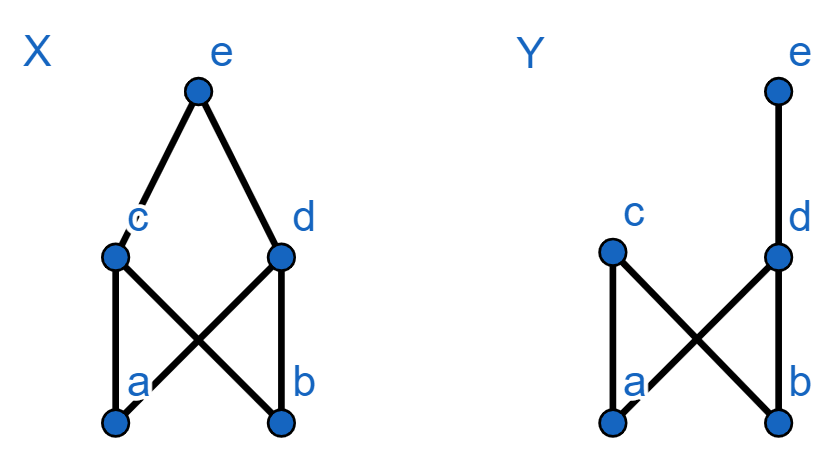
\includegraphics[width=0.5\linewidth]{hasse0.png}
    \end{figure}

    Naslednje zaporedje diagraov, nam pokaže, kako pridemo do jedra prostora $X$, z odstranjevanjem odvečnih točk. Točka $c$ je navzgor odvečna v $X$, $d$ je navzgor odvečna v $X\backslash\{c\}$, $b$ je navzgor odvečna v $X\backslash\{d,c\}$, $e$ je pa navzdol odvečna v $X\backslash\{d,c,b\}$. Prostor $\{a\}$ je minimalen končen prostor in je jedro od $X$. Vidimo, da je $X$ kontraktibilen.
    
    \begin{figure}[h!]
        \centering
        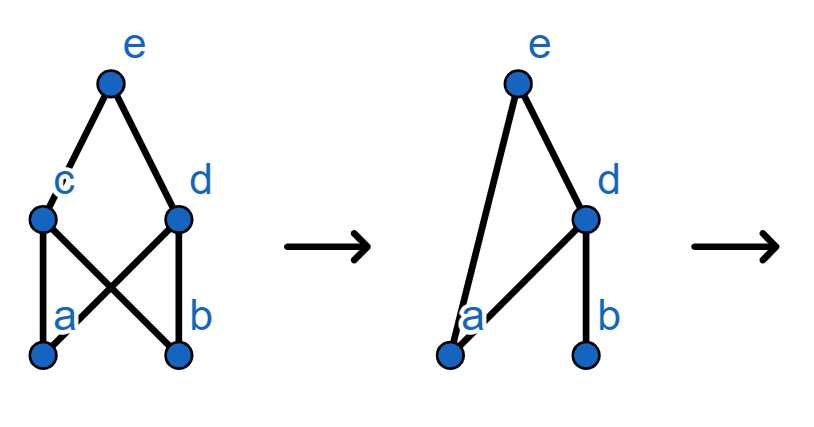
\includegraphics[width=0.5\linewidth]{hasse1.png}
    \end{figure}
     
    \begin{figure}[h!]
        \centering
        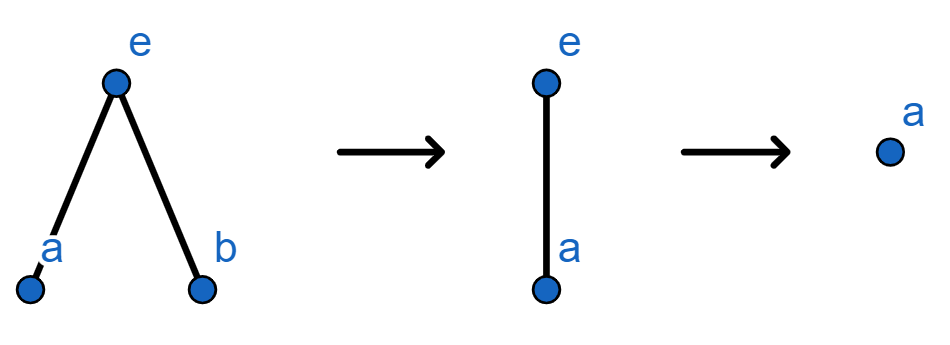
\includegraphics[width=0.5\linewidth]{hasse2.png}
    \end{figure}

    Po drugi strani pa je $e$ navzdol odvečna v $Y$ in $Y\backslash \{e\}$ je minimalen. $X$ in $Y$ nista homotopsko ekvivalentna, saj njuni jedri nista homeomorfni.
    

    
\end{primer}

%\begin{trditev}
%Naj bo $X$ končen $T_0$ prostor, potem je $X$ minimalen končen prostor, natanko tedaj, ko če $\forall x,y\in X$ velja, da če je  $\forall z\in X$ ki je primerljiv z $x$, primerljiv tudi z $y$, potem sledi da $x=y$
%\end{trditev}

%\begin{dokaz}
   
   % Najprej negiramo obe strani ekvivalence. predpostavimo, da $X$ ni minimalen, potem obstaja odvečna točka $x$. Brez škode za splošnost predpostavimo, da je $x$ navzdol odvečna in naj bo $y$ maksimum od $\widehat{U}_x$. Če $z\geq x$, potem je $z\geq y$, če pa je $z\le x$, potem je $z\leq y$, ampak $x\neq y$.
%Recimo zdaj, da obstajata $x\neq y$, taka da je vsak element ki je primerljiv z $x$ primerljiv tudi z $y$, torej je tudi $x$ primerljiv z $y$. Predpostavimo $x>y$. Naj bo $A=\{z\in X |  z>x \text{ in za vsak $w\in X$, primerljiv z $z$, $z$ je primerljiv z $y$}\}$. $A$ je neprazna, saj je $x\in A$. Naj bo $x'$ minimalni element v $A$. Pokažimo, da je $x'$ navzdol odvečna točka in $y=\text{max}(\widehat{U}_x)$. Naj bo zdaj $z<x'$, potem je $z$ primerljiv $y$, saj $x'\in A$. Recimo, da $z>y$ in naj bo $w\in X$. Če $w\geq z$, potem je $w\geq y$, torej $z\in A$, kar je pa v protislovju z minimalnostjo $x'$. Zato $z\leq y$, torej je $y$ maksimum v $\widehat{U}_x$.
%\end{dokaz}

\section{McCordova preslikava}\label{sec:minimal}

\begin{definicija}
    Končni topološki prostor je \textit{model} prostora $X$, če mu je šibko homotopsko ekvivalenten. Model je \textit{minimalen}, če ima izmed vseh modelov najmanjšo kardinalnost.
\end{definicija}


\begin{definicija}
    Naj bo $X$ končen $T_0$ prostor. \textit{Simplicialni kompleks} $\mathcal{K}(X)$ \textit{prirejen X}, je simplicialni kompleks, čigar simpleksi so neprazne verige v $X$. Če je $f\colon  X\rightarrow Y$ zvezna preslikava med dvema $T_0$ prostoroma, je \textit{prirejena simplicialna preslikava} $\mathcal{K}(f)\colon \mathcal{K}(X) \rightarrow \mathcal{K}(Y)$ definirana kot $\mathcal{K}(f)(A) = f(A)$, kjer je  $A\in \mathcal{K}(X)$ veriga $A=\{v_0,v_1,\cdots v_n\}$ in $f(A)=\{f(v_0),f(v_1),\cdots f(v_n)\}$.
\end{definicija}

Vidimo, če je $f\colon  X\rightarrow Y$ zvezna, je $\mathcal{K}(f)\colon \mathcal{K}(X) \rightarrow \mathcal{K}(Y)$ simplicialna, saj je monotona in slika verige v verige.
Točka $\alpha$ v geometrijski realizaciji $|\mathcal{K}(X)|$ je
konveksna kombinacija oblike
$\alpha = \alpha_1 v_1+\alpha_2v_2 + \ldots + \alpha_r v_r$, pri čemer 
$\sum_{i=1}^{r}\alpha_i=1$, $\alpha_i \ge 0$ in 
velja, da je $v_1 < v_2 < \ldots < v_r$ veriga v $X$.
Nosilec $\alpha$ je množica supp($\alpha$)$= \{v_1,v_2,\ldots,v_r\}$. Pomembno vlogo igra 
 preslikava $\alpha \mapsto v_1$.

 \begin{definicija}
    Naj bo $X$ končen $T_0$ prostor, Definirajmo
    \textit{McCordovo} preslikavo $\mu_X\colon |\mathcal{K}
    (X)|\rightarrow X$, z $\mu_X(\alpha) =$
    \text{min}(\text{supp}($\alpha))$.
\end{definicija}



\begin{izrek}{\textbf{McCord}} %opomba???
    Naj bo $X$ splošen in $Y$ končen topološki prostor in naj bo $f\colon X\rightarrow Y$ zvezen. Če je zožitev
    $$
    f|_{f^{-1}(U)}\colon f^{-1}(U)\rightarrow U
    $$
    šibka homotopska ekvivalenca za vsako minimalno odprto množico $U\subseteq$, je $f\colon X\rightarrow Y$  šibka homotopska ekvivalenca.
\label{iz:mccord}
\end{izrek}


%\begin{opomba}
%    Izrek ne velja le za zožitev na bazne množice, ampak tudi na vsako \textit{bazi podobno pokritje}, torej za vsako pokritje, ki je baza za kako drugo topologijo.
%\end{opomba}



\begin{lema}
    Naj bo $x\in X$ in naj bo $L=\mathcal{K} (X\ \backslash \ U_x) \subseteq \mathcal{K}(X)$. Potem se vsak $\alpha \in |\mathcal{K}(X)|\ \backslash \ |L|$ da napisati, kot $\alpha = t\beta + (1-t)\gamma$, za $\beta \in |\mathcal{K}(U_x)|, \ \gamma \in |L|$ in $0<t\leq 1$, pri čemer je $\alpha$ zvezno odvisna od $\beta, \gamma$ in $t$. Koeficienti $\beta, \gamma$ in $t$ so enolično določeni.
\label{lem:sibka}
\end{lema}

\begin{dokaz}
    $L$ je subkompleks, ki ga napenjajo oglišča, ki niso v $U_x$. Za vsak $\alpha \in |\mathcal{K}(X)|\ \backslash \ |L|$, 
    $$\alpha = \sum_{i=1}^{n} \alpha_i v_i 
    = \sum_{i=1}^{r} \alpha_i u_i + \sum_{i=r+1}^{n}\alpha_i v_i,\ \text{za}\ \sum_{i=1}^{n} \alpha_i=1,
    $$
    za $u_i \in U_x$, $v_i \in X \ \backslash \ U_x$ in za nek $r\in \{1,2, \cdots, n-1\}$. S t označimo $\sum_{i=1}^{r} \alpha_i$, torej je $1-t=\sum_{i=r+1}^{n} \alpha_i$ in $0<t\leq 1$. Potem $\beta =\sum_{i=1}^{r} \alpha_i u_i/t \in |\mathcal{K}(U_x)|$, saj je $\sum_{i=1}^{r} \alpha_i/t=1$ in podobno $\gamma=\sum_{i=r+1}^{n} 
    \alpha_i v_i/(1-t) \in |\mathcal{K}(X \ \backslash \ U_x)|$. Zveznost in enoličnost sledi iz konstrukcije.

\end{dokaz}

\begin{izrek}
    \textit{McCordova} preslikava je šibka homotopska 
    ekvivalenca za vsak končen $T_0$-prostor.
    \label{iz:ksibka}
\end{izrek}

\begin{dokaz}
    Definirajmo retrakcijo $r\colon U_x\rightarrow \{x\}$ kot 
    $r(y)=x$, za vsak $y\in U_x$. Ker je $x$ maksimum v 
    $U_x$, je $r\geq 1_X$, zato je po trditvi 
    \ref{iz:ograje} $r\simeq 1_X$, torej je $U_x$ 
    kontraktibilna množica. Dokazali bomo, da je za vsak 
    $x\in X$, $\mu_X^{-1}(U_x)$ odprta in kontraktibilna. S 
    tem bomo pokazali, da je $\mu_X$ zvezna in da so 
    zožitve $\mu_X|_{\mu_X^{-1}(U_x)}\colon \mu_X^{-1}(U_x)\rightarrow 
    U_x$ šibke homotopske ekvivalence, kar pa po McCordovem izreku \ref{iz:mccord}
    pomeni, da je preslikava $\mu_X$ šibka homotopska ekvivalenca.

    Naj bo $x\in X$ in naj bo $L=\mathcal{K}(X\ \backslash \
    U_x)\subseteq \mathcal{K}(X)$. $L$ je torej 
    subkompleks, ki ga napenjajo oglišča, ki niso v $U_x$. 
    Trdimo, da 
    $$
    \mu_X^{-1}(U_x)=|\mathcal{K}(X)|\ \backslash \ |L|.
    $$
    Pokažimo najprej, da $\mu_X^{-1}(U_x)\subseteq 
    |\mathcal{K}(X)|\ \backslash \ |L|$. Naj bo $\alpha \in 
    \mu_X^{-1}(U_x)$, torej je min$(\text{supp}
    (\alpha))\in U_x$, zato \text{supp}($\alpha$) vsebuje 
    oglišče iz $U_x$, zato $\alpha \notin |L|$, torej $\alpha 
    \in |\mathcal{K}(X)|\ \backslash \ |L|$.

    Pokažimo še, da $|\mathcal{K}(X)|\ \backslash \
    |L|\subseteq \mu_X^{-1}(U_x)$. Naj $\alpha \in |\mathcal{K}(X)|\ \backslash \ |L|.$
    Če  $\alpha \notin |L|$, potem obstaja $y\in 
    \text{supp}(\alpha)$, tak, da $y \in U_x$, zato je 
    min$(\text{supp}(\alpha))\leq y \leq x$, zato je 
    $\mu_X(\alpha) \in U_x$ in $\alpha \in \mu_X^{-1}
    (U_x)$.
    Ker je $|L|$ zaprta podmnožica $|\mathcal{K}(X)|$, je 
    $\mu_X^{-1}(U_x)$ odprta.

    Pokažimo, da je $\mu_X^{-1}(U_x)$ kontrabilna. Prvo pokažimo, da je 
    $|\mathcal{K}(U_x)|$ krepki deformacijski retrakt 
    od $|\mathcal{K}(X)|\ \backslash \ |L|$. Naj bo $i\colon |\mathcal{K}(U_x)|\hookrightarrow |\mathcal{K}
    (X)|\ \backslash \ |L|$ inkluzija. Če je $\alpha \in |\mathcal{K}(X)|\ 
    \backslash \ |L|$, potem je po lemi \ref{lem:sibka}  $\alpha = t\beta + 
    (1-t)\gamma$, za $\beta \in |\mathcal{K}(U_x)|, \ \gamma \in |L|$ in $0<t\leq 1$. 
    Definirajmo $r\colon |\mathcal{K}(X)|\ \backslash \ |L|\rightarrow |\mathcal{K}(U_x)|$ 
    kot $r(\alpha)=\beta$. Ker je $\alpha$ zvezna in je zožitev $r|_{(|\mathcal{K}(X)|\ \backslash \ |L|)\cap 
    \overline{\sigma}}\colon (|\mathcal{K}(X)|\ \backslash \ |L|)\cap 
    \overline{\sigma} \rightarrow |\mathcal{K}(U_x)|$ zvezna, za vsak 
    $\sigma \in \mathcal{K}(X)$, sledi da je $r$ zvezna. Definirajmo zdaj linearno homotopijo $H\colon (|\mathcal{K}(X)|\ \backslash \ |L|) \times I \rightarrow (|\mathcal{K}(X)|\ \backslash \ |L|)$ med $1_{(|\mathcal{K}(X)|\ \backslash \ |L|)}$ in $ir$ kot 
    $$
    H(\alpha,s)=(1-s)\alpha + s\beta.
    $$
    H je dobro definirana, in zvezna, saj je vsaka zožitev 
    $$
    H|_{((|\mathcal{K}(X)|\ \backslash \ |L|)\cap 
    \overline{\sigma})\times I}\colon ((|\mathcal{K}(X)|\ \backslash \ |L|)\cap 
    \overline{\sigma})\times I \rightarrow |\mathcal{K}(U_x)|
    $$
    dobro definirana in zvezna, za vsak $\sigma \in \mathcal{K}(X)$.

    Ker je vsak element iz $U_x$ primerljiv z $x$, je $\mathcal{K}(U_x)$ 
    simplicialni stožec, zato je po trditvi \ref{pos:kontr} $|\mathcal{K}(U_x)|$ 
    kontraktibilen in zato je kontraktibilna tudi $\mu_X^{-1}
    (U_x)=|\mathcal{K}(X)|\ \backslash \ |L|$.
\end{dokaz}


\begin{figure}[h]
    \centering
    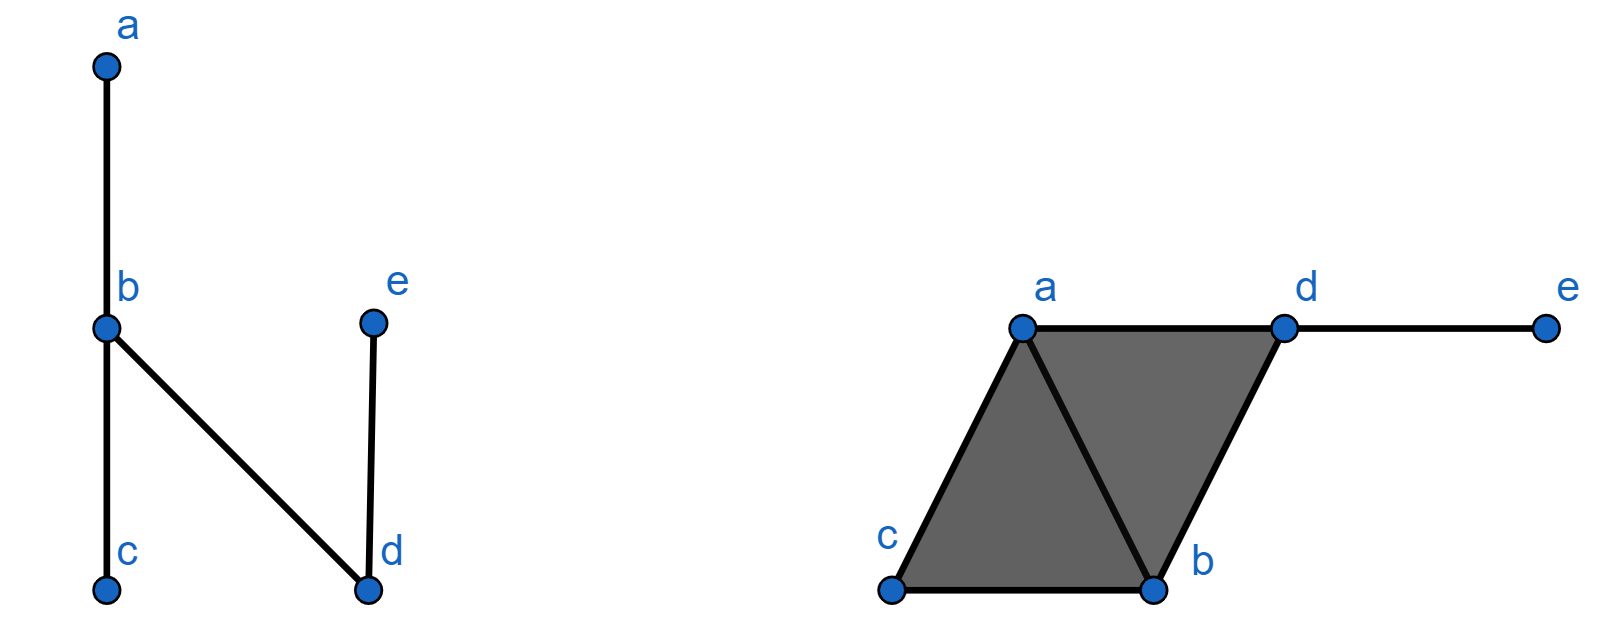
\includegraphics[width=1\linewidth]{simp.png}
    \caption{Končen prostor in geometrijska realizacija prirejenega simplicialni kompleks v $\R^2$, ki mu je šibko homotopsko ekvivalentna.}
\end{figure}
Če imamo končen topološki prostor $X$, mu priredimo simplicialni kompleks
$\mathcal{K}(X)$, Geometrijska realizacija $|\mathcal{K}(X)|$ tega kompleksa pa je šibko homotopsko ekvivalentna 
začetnemu prostoru $X$. Torej lahko za vsak prostor, ki je homeomorfen geometrijski realizaciji
nekega simplicialnega kompleksa, najdemo njegov končen model tj. končen topološki prostor, ki mu
je šibko homotopsko ekvivalenten.




\section{Konstrukcije novih topoloških prostorov}


V tem poglavju bomo definirali nekaj osnovnih konstrukcij iz algebraične topologije in jih uporabili na simplicialnih kompleksih ter končnih in splošnih topoloških prostorih. S $S^n$ označimo $n-$dimenzionalno sfero.

\textit{Spoj} Topoloških prostorov $X$ in $Y$ je topološki prostor $X\ast Y = X\times Y 
\times I /_{\sim}$, pri čemer $(x, y_1, 0) \sim (x, y_2, 0)$ in  $(x_1, y, 1) \sim (x2, y, 1)$. 
Torej $X\times Y\times \{0\}$ strnemo na $X$ in $X\times Y\times \{1\}$ na $Y$. Intuitivno, 
to pomeni, da vsako točko na $X$ z intervalom povežemo z vsako točko na $Y$.
Poseben primer spoja je \textit{suspenzija} $\Sigma X$, ki je spoj $X$ in prostora na dveh točkah, $S^0$.

$$
\Sigma X=S^0\ast X = X\times I /_{(X\times \{0\},X\times \{1\})}
$$

\begin{figure}[h]
    \centering
    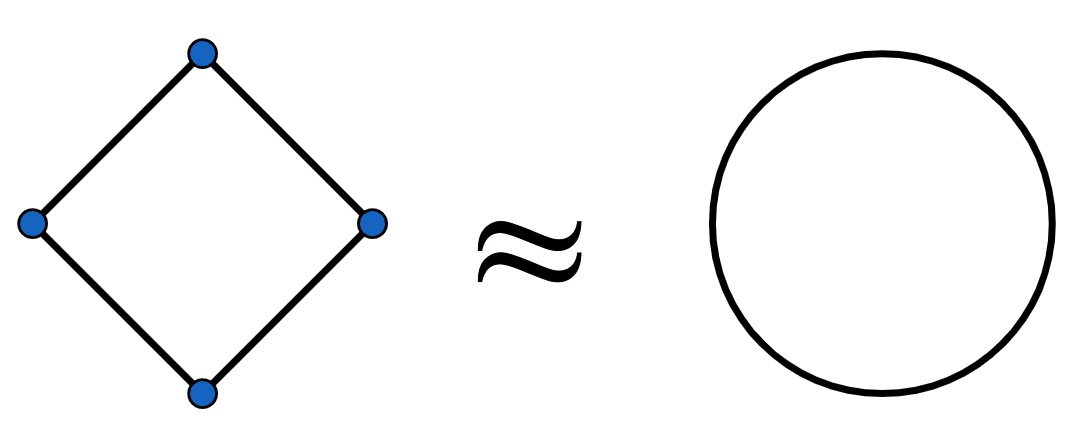
\includegraphics[width=0.6\linewidth]{homeo2.png}
    \caption{Suspenzija $\Sigma S^0$ je homeomorfna $S^1$. V splošnem velja $\Sigma S^n=S^{n+1}$}
\end{figure}

Naj bosta $X$ in $Y$ topološka prostora. Naj $x_0\in X$ in $y_0\in Y$ Potem je 
\textit{šop} $X\bigvee Y$ kvocient disjunktne unije $X\bigsqcup Y$, pri
 katerem identificiramo $x_0$ in $y_0$. Na primer $S^1\bigvee S^1$ je prostor,
  ki ga dobimo, če staknemo dve krožnici v eni točki in je homeomorfen "\textbf{8}".


\textit{Simplicialni spoj $K\ast L$} kompleksov $K$ in $L$ z disjunktnima množicama oglišč je kompleks.

$$
K\ast L=K\cup L \cup \{\sigma \cup \tau| \sigma \in K, \tau \in L \}
$$

\textit{Simplicialni stožec} $aK$ z bazo $K$ je simplicialni spoj $K$ in oglišča $a\notin K$


\begin{trditev}
    Naj bosta $K$ in $L$ končna simplicialna kompleksa, potem je geometrijska realizacija $|K\ast L|$ homeomorfna topološkemu spoju $|K|\ast |L|$.
    \label{tr:spoj}
\end{trditev}

\begin{dokaz}
    Definirajmo $f\colon |K|\times |L|\times I\rightarrow |K\ast L|$, kot $f(k,l,j)=jk+(1-j)l$. Če $k=\Sigma_{i=1}^n \alpha_i v_i$ in $l=\Sigma_{i=1}^m \beta_i u_i$, potem je $\{v_i|\text{ $\alpha_i > 0$}\}$ simpleks v $K$ in $\{u_i|\text{ $\beta_i > 0$}\}$ simpleks v $L$ ter $\Sigma_{i=1}^n \alpha_i = \Sigma_{i=1}^m \beta_i=1$. Zato je $\{v_i|\text{ $\alpha_i > 0$}\}\cup \{u_i|\text{ $\beta_i > 0$}\}$ simpleks v $K\ast L$  in $\Sigma_{i=1}^n \alpha_i j + \Sigma_{i=1}^m \beta_i (1-j)=1$. Torej je $f$ dobro definirana. Velja tudi $f(k,l,0)=l$, neodvisno od $k$ in $f(k',l',1)=k'$, neodvisno od $l'$, torej $f$ slika ekvivalenčne razrede v točke. Ker sta $K$ in $L$ končna kompleksa, je $|K|\times |L|\times I$ kompaktna. Torej $f$ slika iz kompakta v $T_2$ prostor in je zato zaprta. Preslikava $f$ je zaprta in surjektivna, zato je kvocientna. Naredi iste identifikacije kot $q$, zato je inducirana preslikava $\overline{f}$ dobro definirana in je homeomorfizem.
    
\[\begin{tikzcd}
    {|K|\times |L|\times I }\arrow{r}{f} \arrow[swap]{d}{q} & {|K\ast L|} \\
    {|K|\ast |L|} \arrow{ru}{\overline{f}}
   \end{tikzcd}
    \]


\end{dokaz}

Če je $K$ 0-kompleks z dvema ogliščema, potem je $|K\ast L|=|K|\ast |L|=S^0\ast |L| = \Sigma |L|$.

\begin{figure}[h]
    \centering
    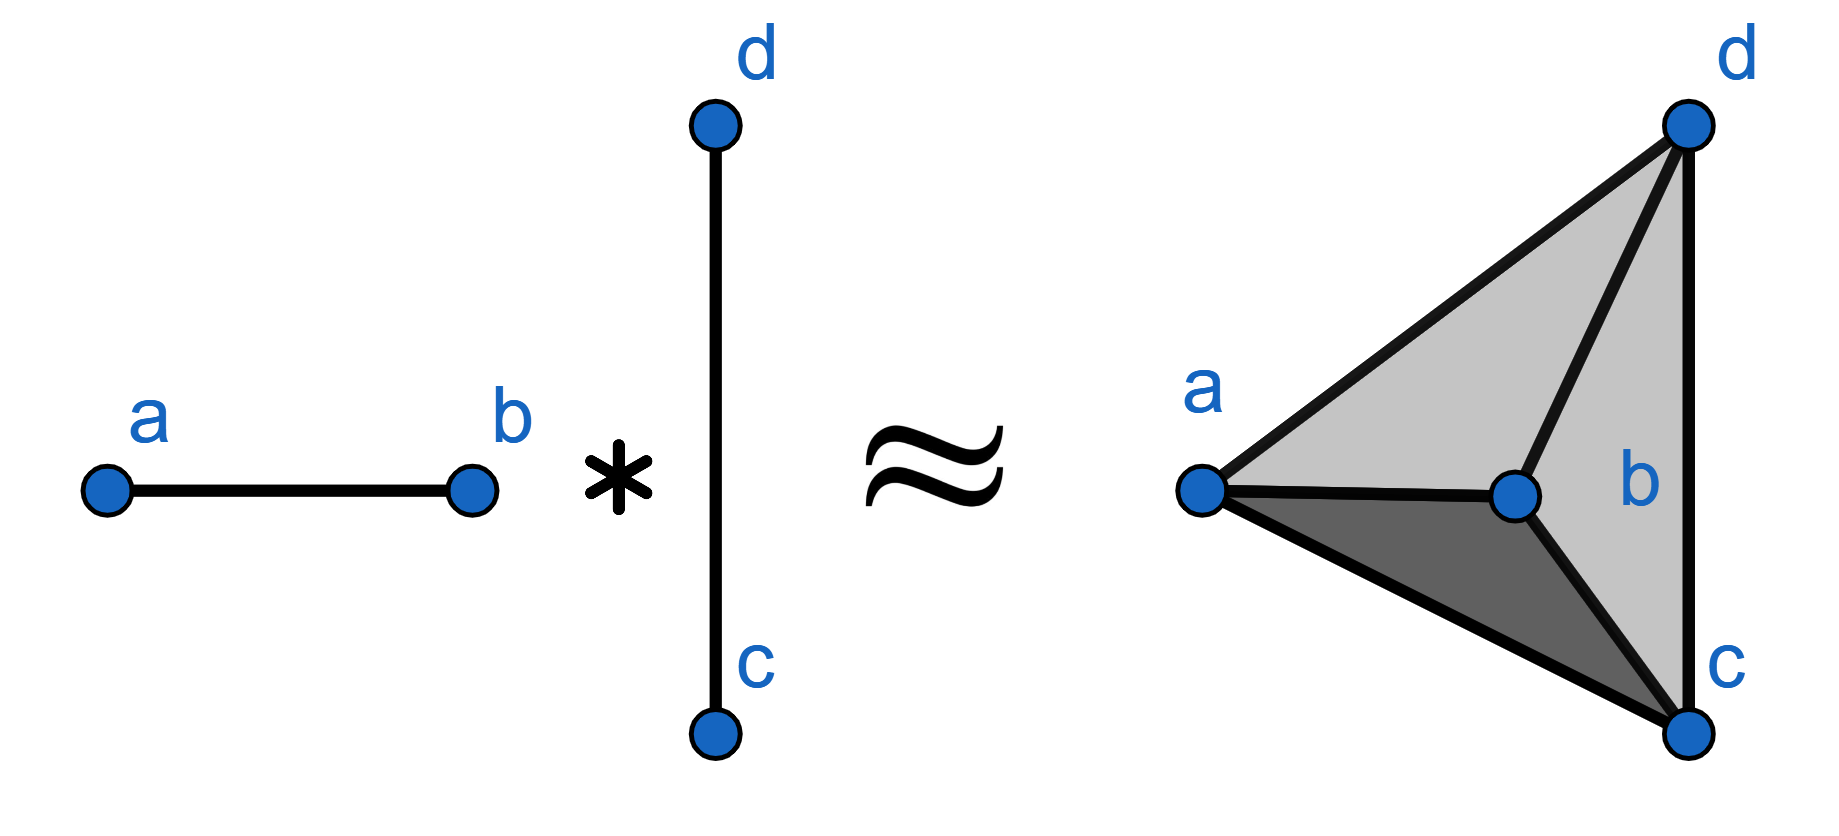
\includegraphics[width=0.6\linewidth]{spoj.png}
    \caption{Geometrijska realizacija simplicialnega spoja dveh $1-$simpleksov je homeomorfna geometrijski realizaciji $3-$simpleksa.}
\end{figure}

\begin{definicija}
    \textit{Ne-Hausdorffov spoj} $X\circledast Y$ dveh končnih $T_0-$prostorov
     $X$ in $Y$, je disjunktna unija $X\bigsqcup Y$, v kateri
     pustimo ureditev v $X$ in v $Y$ in nastavimo $x\leq y$ za vsaka 
     $x\in X$ in $y\in Y$.
\end{definicija}

Ta spoj je asociativen in v splošnem ni komutativen. Tako kot pri topološkem
 in simplicialnem spoju imamo poseben primer ne-Hausdorffovega ne-Hausdorffove Suspenzije
  $\Sus(X)=X \circledast S^0$.

  Ne-Hausdorffova suspenzija reda $n$ je definirana rekurzivno, kot  $\Sus^n=\Sus(\Sus^{n-1}(X))$.
  \begin{opomba}
    Velja $\mathcal{K}(X\circledast Y) = \mathcal{K}(Y)\ast \mathcal{K}(X)$.
    \label{op:spoj}
  \end{opomba}

  \section{Minimalni model sfere}


  \begin{definicija}
      Končni topološki prostor je \textit{model} prostora $X$, če mu je šibko homotopsko ekvivalenten. Model je \textit{minimalen}, če ima izmed vseh modelov najmanjšo kardinalnost.
  \end{definicija}
  
  Spomnimo se, da je minimalni končni prostor, prostor brez odvečnih točk. Ker je pa vsak končen prostor homotopsko ekvivalenten svojemu jedru, sledi, da je vsak minimalni končni model prostora tudi minimalen končen prostor.
  
  \begin{trditev}
      Končen prostor $\Sus^n(S^0)$ je končni model n-dimenzionalne sfere $S^n$ za vsak $n\geq 0$
  \end{trditev}
  
  \begin{dokaz}
      Vemo že, da je $\Sus^n(S^0)$ šibko homotopsko ekvivalenten $|\mathcal{K}(\Sus^n(S^0))|$,\ 
      po opombi\\ \ref{op:spoj} in trditvi \ref{tr:spoj} pa velja $|\mathcal{K}(\Sus^n(S^0))|=|\mathcal{K}(\underbrace{S^0\circledast S^0 \circledast \cdots \circledast S^0}_\text{$n+1$-krat})|=
      |\mathcal{K}(S^0)\ast\mathcal{K}(S^0) \ast \cdots \ast \mathcal{K}(S^0)|=|\mathcal{K}(S^0)|\ast
      |\mathcal{K}(S^0)| \ast \cdots \ast |\mathcal{K}(S^0)|=S^0\ast
      S^0 \ast \cdots \ast S^0=S^n$
  \end{dokaz}

  Zdaj bomo še dokazali, da je $\Sus^n(S^0)$ minimalni končni model za $S^n$. Še več, pokazali bomo, da ima vsak prostor, šibko homotopsko ekvivalenten $S^n$ vsaj $2n+2$ točk. Če ima pa natanko $2n+2$ točk pa je homeomorfen $\Sus^n(S^0)$.

  \begin{definicija}
      \textit{Višina} $\htt(X)$ končne delno urejene množice je ena manj kot dožina najdaljše verige v $X$. Z $\# X$ pa označimo število elementov v $X$.
  \end{definicija}
  Dimenzija prirejenega kompleksa $\mathcal{K}(X)$ je enaka $\htt(X)$.
  
  
  \begin{izrek}
      Naj bo $X\neq\ast$ minimalen prostor, potem ima vsaj $2\htt(X)+2$ točk. Če ima natanko $2\htt(X)+2$ točk, potem je homeomorfen $\Sus^{\htt(X)}(S^0)$
  \end{izrek}    
  
  \begin{dokaz}
      Naj bo $x_0<x_1 <\cdots <x_h$ veriga dolžine $h+1$ za $h=\htt(X)$. Ker je $X$
       minimalen, $x_i$ ni odvečna točka za noben $0\leq i <h$. Potem za 
       vsak $0\leq i <h$ obstaja $y_{i+1}$, tak da $y_{i+1}> x_i$ in $y_{i+1}
       \ngeq x_{i+1}$ $(1)$. Trdimo, da so vse točke $y_i$ med seboj različne, za vsak
        $0< i \leq h$ in da nobena ni enaka $x_j$ za noben $0\leq j \leq h$.
  


        Ker $y_{i+1} > x_i$, sledi, da $y_{i+1}\neq x_j$ za noben $j\leq i$. Ker velja tudi $y_{i+1}\ngeq x_{i+1}$ pa sledi, da $y_{i+1}\neq x_j$ za 
        noben $j> i$.
  
        Če je $y_{i+1}= y_{j+1}$ za nek $i<j$, potem je $y_{i+1}= y_{j+1}\geq
         x_j \geq x_{i+1}$. To je pa v protislovju z $y_{i+1} 
         \ngeq x_{i+1}$.
  
         Ker je vsak končen prostor z minimumom ali z maksimumom kontraktibilen 
         in je $X\neq \ast$, minimalen prostor, sledi da $X$ nima minimuma. Zato mora obstajati točka $y_0\in X$, za katero velja $y_0 \ngeq x_0$.

         \begin{figure}[h!]
            \centering
            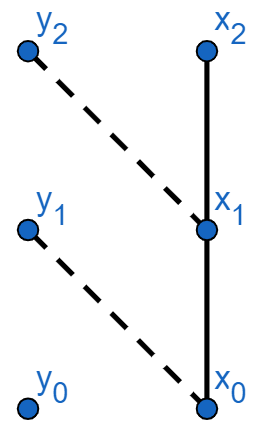
\includegraphics[width=0.2\linewidth]{minsfera-prva.png}
          \caption{Dokaz je morda malo zahtevnejši, zato ga bomo demonstrirali na primeru, ko je višina $X$ enaka 2. Če je $X$ višine 2, imamo verigo $x-$ov dolžine 3. Točki $y_1$ in $y_2$ morata obstajata, ker $x_0$ in $x_1$ nista navzgor odpravljiva. Točka $y_0$ pa obstaja, ker $X$ ni kontraktibilen prostor.}
          \end{figure}


          Zato je $y_0$ različna od drugih $2h+1$ točk in zato $\# X\geq 2h+2$.
          Predpodstavimo zdaj, da ima $X$ natanko $2h+2$ točk, torej 
          $$
          X=\{x_0,x_1,\cdots x_h,y_0,y_1,\cdots y_h,\}.
          $$
          Če bi bil $x_i > y_i$, za $0<i\leq h$ bi bilo to v nasprotju z 
          maksimalnostjo verige $x_0 <\cdots <x_h$, saj bi potem veljalo $x_{i-1} 
          < y_i < x_i$. Tudi $y_i \ngtr x_i$ za $0\leq i \leq h$ zaradi (1), zato sta $x_i $ in $y_i$ neprimerljiva za $0\leq i \leq h$.
  

          \begin{figure}[h!]
            \centering
            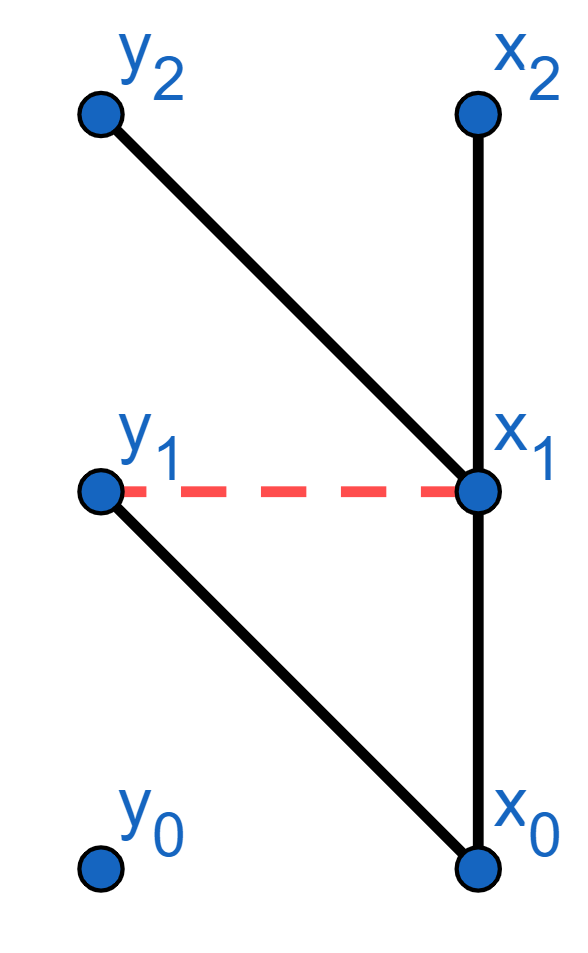
\includegraphics[width=0.2\linewidth]{minsfera_vodoravna.png}
          \caption{$x_1$ ni večji od $y_1$, saj bi potem imeli verigo dolžine 4, $x_0<y_1<x_1<x_2$. Tudi $y_1$ ni večji od $x_1$, saj potem v Hassejevem diagramu ne bi bilo povezave med $x_0$ in $x_1$. Torej sledi, da v diagramu ni vodoravnih povezav.}
          \end{figure}

          Z indukcijo na $j$ pokažimo, da $y_i < x_j$ in $y_i < y_j$ za vse $i<j$. Za $j=0$ 
          ni kaj za dokazovati. Naj bo $0\leq k <h$ in recimo, da trditev drži za $j=k$, 
          dokažimo, da drži tudi za $j=k+1$. Ker $x_{k+1}$ ni navzdol odvečna, 
          obstaja $z$, da $z< x_{k+1}$ in $z\nleq x_k$. Ker sta $x_{k+1}$ in 
          $y_{k+1}$ neprimerljiva, velja tudi $z\neq y_{k+1}$. Iz indukcijske 
          predpodstavke sledi, da je vsaka točka, z izjemo $y_k$ in $y_{k+1}$, večja 
          od $x_{k+1}$ ali manjša od $x_k$. Ker $y_{k+1} \nleq x_{k+1}$, je potem
          $z=y_k$ in zato $y_k<x_{k+1}$. Dokažimo še, da $y_k\leq y_{k+1}$. Ker 
          $y_{k+1}$ ni navzdol odvečna, obstaja $w\in X$, da je $w<y_{k+1}$ in 
          $w\nleq x_k$. Iz indukcijske predpodstavke
           in dejstva, da $y_{k+1}\ngeq x_{k+1}$, sklepamo,
          da $w=y_k$ in zato $y_k<y_{k+1}$. Za $i<k$ pa velja $y_i<x_k<x_{k+1}$ in
          $y_i<x_k<y_{k+1}$.


          
          \begin{figure}[h!]
            \centering
            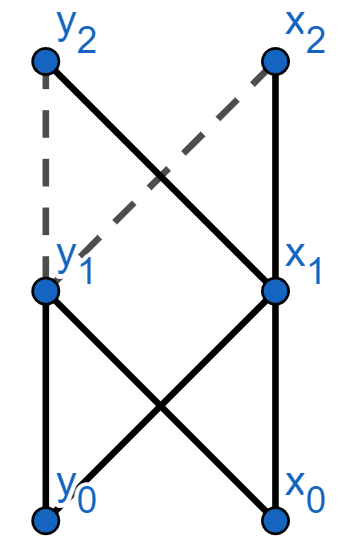
\includegraphics[width=0.2\linewidth]{minsfera-zadnja.png}
          \caption{Pokažimo inducijski korak iz $j=1$ v $j=2$. Ker $x_2$ in $y_2$ nista navzdol odvečni, obstajata $w<x_2$ in $z<y_2$. Edina možna izbira za $w$ in $z$ je $y_1$, torej $y_1<x_2$ in $y_1<y_2$}
          \end{figure}
  
          Dokazali smo, da za vsak $i<j$,  velja $y_i < x_j,\ y_i < y_j,\ x_i < x_j$ in
$x_i < y_j$ ter da sta $x_i$ in $y_i$ neprimerljiva za vsak $0\leq j \leq h$.
To je pa ureditev v $\Sus^h(S^0)$ in zato je $X$ homeomorfen 
    $\Sus^h(S^0)$.
  
\end{dokaz}

\begin{figure}[h]
    \centering
    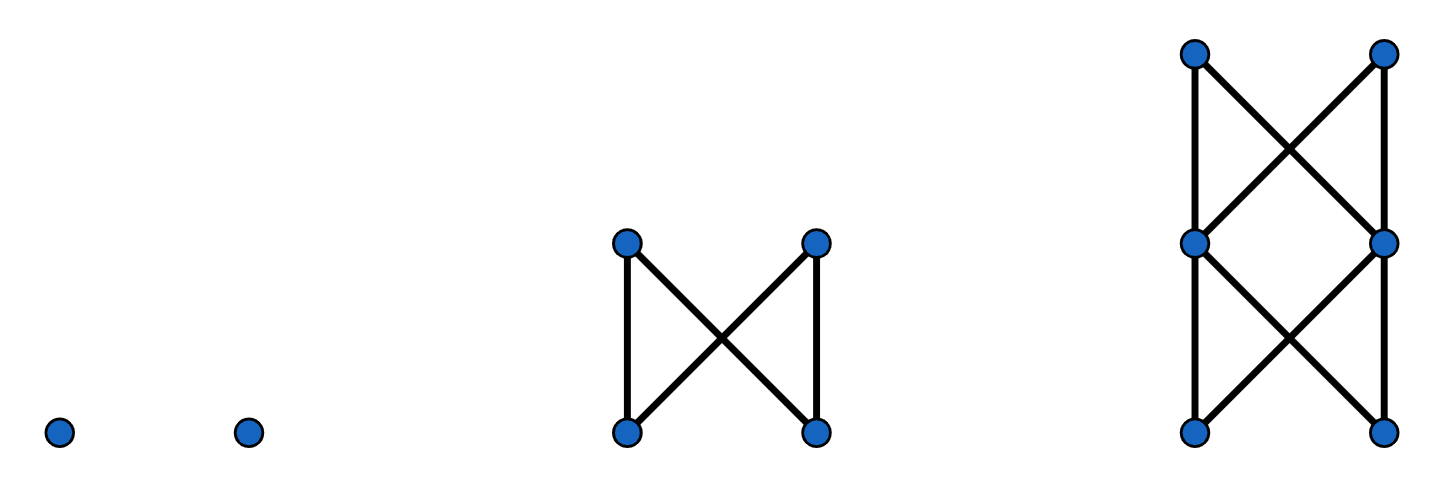
\includegraphics[width=0.8\linewidth]{sfere.png}
    \caption{Minimalni modeli za $S^0$, $S^1$ in $S^2$.}
\end{figure}

Ker je $\Sus^n(S^0)$ model za $S^n$, čigar višina je enaka $n$ in ima 
$2n+2$ točk, je $\Sus^n(S^0)$ minimalni model za $S^n$. Model je 
enoličen, saj je vsak model za $S^n$ na $2n+2$ točkah homeomorfen 
$\Sus^n(S^0)$.
\section{Zanke v Hassejevem diagramu}\label{sec:hasse}

Pokazali bomo, kako se fundamentalna grupa končnega $T_0$ 
prostora izraža preko prirejenega Hassejevega diagrama.
Hassejev diagram končnega $T_0$ prostora $X$ označimo z 
$\h(X)$, z $E(\h(X))$ pa označimo množico njegovih robov.


\begin{definicija}
    Naj bo $(X,x_0)$ končen$T_0$ prostor z izhodiščno točko. Urejen par 
$e=(x,y)$ imenujemo $\mathcal{H}-$rob od $X$, če $(x,y)\in 
E(\mathcal{H}(\mathcal{X}))$, ali $(y,x)\in 
E(\h(X))$. Točki $x$ rečemo \textit{začetek} $x$ in označimo 
$x=\mathfrak{o}(e)$, točki $y$ pa \textit{konec} od $e$, 
označimo $\mathfrak{e}(e)=y$. \textit{Inverz} $\h-$roba $e=(x,y)$ je $\h-$rob $e^{-1}=(y,x)$.

$\h-$pot v $(X,x_0)$ je zaporedje (lahko tudi prazno), $\h-$robov $\xi=e_1e_2\cdots e_n$, 
za katerega velja, da je $\mathfrak{e}(e_i)=\mathfrak{o}(e_{i+1})$, za vsak $0\leq i \leq n-1$.
 Začetek $\h-$poti $\xi$ je  $\mathfrak{o}(\xi)=e_1$, konec pa $\mathfrak{e}(\xi)=e_n$.
 Začetek in konec prazne poti je $\mathfrak{o}(\emptyset)=\mathfrak{e}(\emptyset)=x_0$.
 Če je $\xi=e_1,e_2\cdots e_n$ $\h-$pot, definiramo $\overline{\xi}=e_n^{-1},\cdots 
 e_2^{-1}e_n^{-1}$. Če sta $\xi$ in $\xi'$ $\h-$poti in velja $\mathfrak{e}(\xi)=
 \mathfrak{e}(\xi')$, lahko definiramo produktno \pot $\xi\xi'$, kot zaporednje 
 $\h-$robov v $\xi$, ki mu sledi zaporednje $\h-$robov v $\xi'$.

 Za \pot $\xi=e_1e_2,\cdots e_n$ pravimo, da je \textit{monotona}, če je $e_i\in 
 E(\h(X))$ za vsak $1\leq i \leq n$ ali pa je $e_i^{-1}\in E(\h(X))$ za vsak $1\leq i \leq n$.
 \textit{Zanka} iz $x_0$ je \pot, ki se začne in konča v $x_0$. Za zanki $\xi$ in
  $\xi'$ rečemo, da sta blizu, če obstajajo monotone $\h-$poti $\xi_1,\xi_2,\xi_3,\xi_4$,
   take, da  sta množici $\{\xi,\xi'\}$ in $\{\xi_1\xi_2\xi_3\xi_4,\xi_1\xi_4\}$ enaki.

   Rečemo, da sta zanki $\xi$ in $\xi'$ $\h-$ekvivalentni, če obstaja končno zaporednje zank $\xi=\xi_1,\xi_2, \cdots ,\xi_n=\xi'$, tako da sta vsaki zaporedni zanki blizu. Z $\langle\xi\rangle$ označimo $\h-$ ekvivalenčni razred zanke $\xi$ in z $\mathscr{H}(X,x_0)$ množico teh razredov.
\end{definicija}

\begin{figure}[h!]
    \centering
    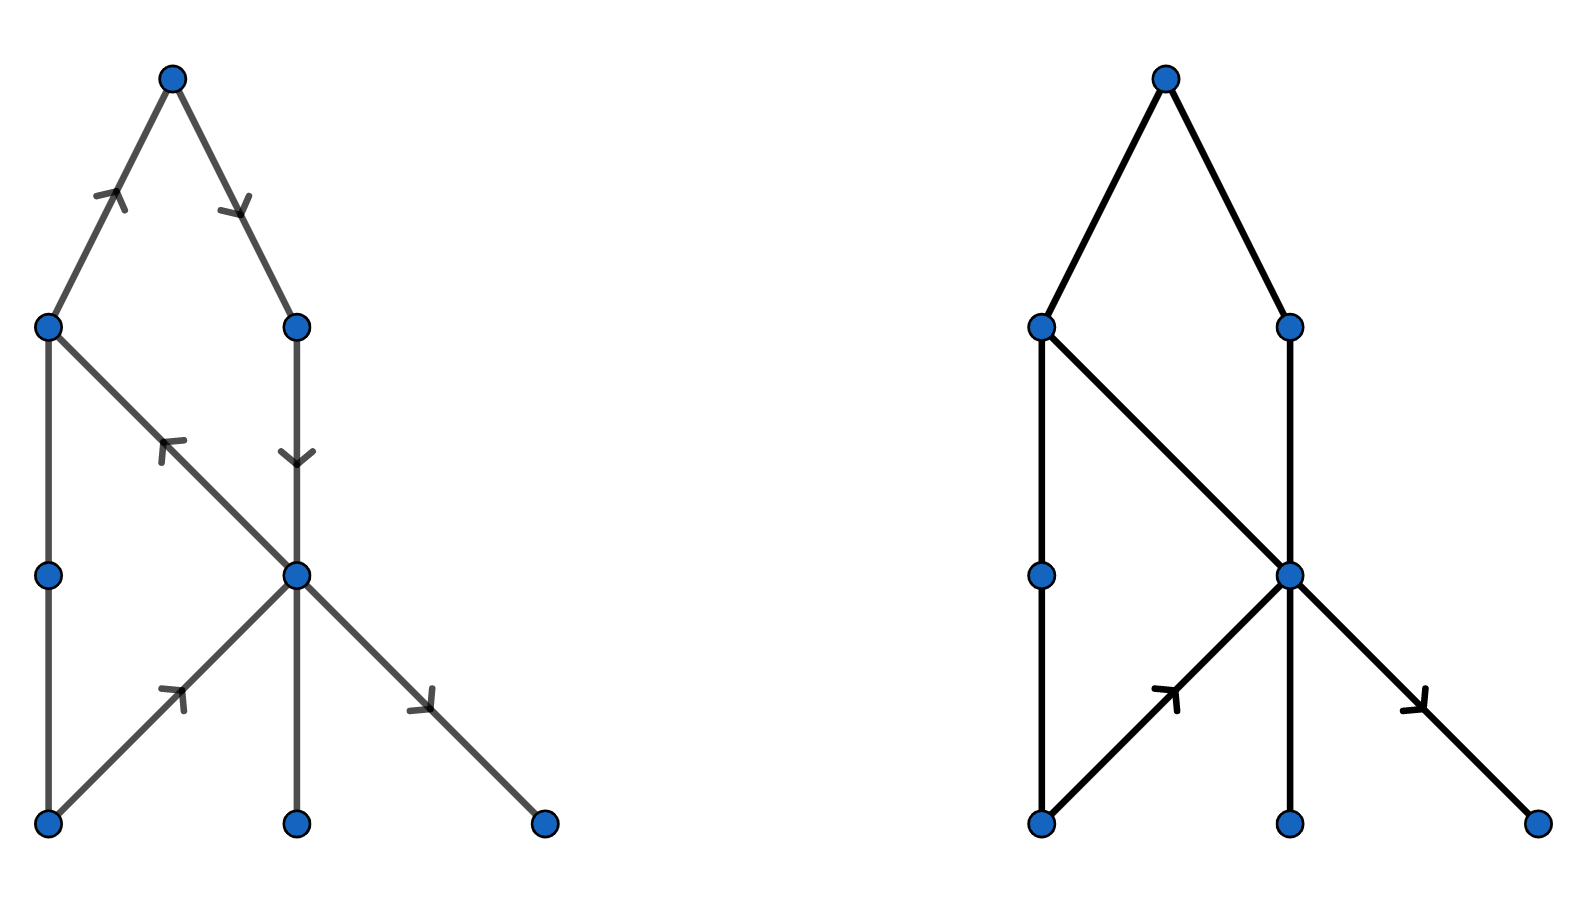
\includegraphics[width=0.6\linewidth]{poti.png}
  \caption{Primer poti ki sta blizu}
  \end{figure}

\begin{izrek}
Naj bo $(X,x_0)$ končen $T_0$ prostor z izhodiščno točko. Potem je množenje $\langle\xi\rangle\langle\xi'\rangle=\langle\xi\xi'\rangle$ dobro definirano in inducira grupno strukturo na $\mathscr{H}(X,x_0)$
\end{izrek}

\begin{dokaz}
Dobra definiranost in asociativnost sta očitni, enota je $\langle\emptyset\rangle$. Naj bosta $\xi$ in $\xi'$ poti, $e$ $\h-$rob in $\mathfrak{e}(\xi)=\mathfrak{o}(\xi')=\mathfrak{o}(e)$ ter $\mathfrak{o}(\xi)=\mathfrak{e}(\xi)=x_0$. Potem sta zanki $\langle\xi \xi'\rangle$ in $\langle\xi e e^{-1} \xi'\rangle$ blizu, saj je $e$ monotona pot. Iz tega takoj sledi, da je inverz od $\langle e_1 e_2 \cdots e_n\rangle$ enak $\langle e_n^{-1} \cdots e_2^{-1}e_1^{-1}\rangle$.
\end{dokaz}


\begin{izrek}
Naj bo $(X,x_0)$ končen $T_0$ prostor z izhodiščno točko. Potem je grupa sklenjenih lomljenk $E(\mathcal{K}(X),x_0)$ izomorfna $\mathscr{H}(X,x_0)$.
\end{izrek}

\begin{dokaz}
    Definirajmo 
    \begin{align*}
\varphi\colon \mathscr{H}(X,x_0)&\rightarrow E(\mathcal{K}(X),x_0)\\
\langle e_1e_2 \cdots e_n\rangle&\mapsto [e_1e_2 \cdots e_n]\\
\emptyset &\mapsto [(x_0,x_0)]
    \end{align*}.

    Najprej pokažimo, da je $\varphi$ dobro definiran.
    Naj bosta zanki $\xi_1 \xi_2 \xi_3 \xi_4$ in $\xi_1 \xi_4 $ blizu in naj bosta $\xi_2 = e_1e_2 \cdots e_n$ in $\xi_3 = e'_1e'_2 \cdots e'_m$ monotoni $\h-$poti. Potem velja 
\begin{align*}
    [\xi_1 \xi_2 \xi_3 \xi_4]&=[\xi_1 e_1e_2 \cdots e_{n-1}(\mathfrak{o}(e_n)\mathfrak{e}(e_n)) \xi_3 \xi_4]\\
    &=[\xi_1 e_1e_2 \cdots e_{n-2}(\mathfrak{o}(e_{n-1})\mathfrak{e}(e_n)) \xi_3 \xi_4]=\cdots=[\xi_1(\mathfrak{e}(\xi_1)\mathfrak{e}(e_n)) \xi_3 \xi_4],
\end{align*}
saj je $\{\mathfrak{o}(e_{n-i-1}),\mathfrak{o}(e_{n-i}),\mathfrak{e}(e_{n})\}$ simpleks v $\mathcal{K}(X)$, analogno 
$$
[\xi_1(\mathfrak{e}(\xi_1)\mathfrak{e}(e_n)) \xi_3 \xi_4]=[\xi_1(\mathfrak{e}(\xi_1)\mathfrak{e}(e_n))( \mathfrak{o}(e'_1)\mathfrak{o}(\xi_4)) \xi_4]
$$
in zato 
\begin{align*}
    [\xi_1 \xi_2 \xi_3 \xi_4]&=[\xi_1(\mathfrak{e}(\xi_1)\mathfrak{e}(e_n)) (\mathfrak{o}(e'_n)\mathfrak{o}(\xi_4)) \xi_4]\\
    &=[\xi_1(\mathfrak{e}(\xi_1)\mathfrak{e}(e_n)) (\mathfrak{e}(e_n)\mathfrak{e}(\xi_1)) \xi_4]=[\xi_1(\mathfrak{e}(\xi_1) \mathfrak{e}(\xi_1)) \xi_4]=[\xi_1 \xi_4].
\end{align*}


Obratno, če je $\xi =(x_0,x_1)(x_1,x_2) \cdots (x_{n-1},x_n)$ lomljenka v $\mathcal{K}(X)$ z $x_0=x_n$, potem sta $x_i$ in $x_{i-1}$ primerljiva za vsak $1\leq i \leq n$. Zato lahko najdemo monotone $\h-$poti $\xi_1, \xi_2, \cdots  \xi_n$, take da $\mathfrak{o}(x_{i-1})=\mathfrak{e}(x_i)$ za $1\leq i \leq n$. Definirajmo

\begin{align*}
    \psi\colon  E(\mathcal{K}(X),x_0)&\rightarrow \mathscr{H}(X,x_0),\\
    [\xi]&\mapsto \langle\xi_1, \xi_2, \cdots  \xi_n\rangle.
\end{align*}

Definicija je neodvisna od izbire $\h-$poti $\xi_i$, saj če se izbiri razlikujeta za kak $i=k$, potem sta $\xi_1 \cdots \xi_k \cdots \xi_n$ in $\xi_1 \cdots \xi'_k \cdots \xi_n$ $\h-$ekvivalentni, saj sta obe blizu $\xi_1 \cdots \xi_k\xi_k^{-1}\xi'_k \cdots \xi_n$- Zato $\langle \xi_1 \cdots \xi_k \cdots \xi_n \rangle = \langle \xi_1 \cdots \xi'_k \cdots \xi_n \rangle$.

Definicija je neodvisna od izbire predstavnika. Recimo da sta $\xi(x,y)(y,z)\xi'$ in $\xi(x,z)\xi'$ ekvivalentni lomljenki v $\mathcal{K}(X)$, ki se začneta in končata v $x_0$, pri čemer sta $\xi$ in $\xi'$ lomljenki, $x,y$ in $z$ pa so primerljivi.
Če $y$ leži med $x$ in $z$, lahko najdemo monotono $\mathcal{H}-$pot od $x$ do $z$, ki vsebuje $y$ in nadomesti \pot od $x$ do $y$ in od $y$ do $z$. Zato je $\psi$ ekvivalentno definirana na $\xi(x,y)(y,x)\xi'$ in $\xi(x,z)\xi'$.
Če je $z\leq x \leq y$ lahko poiščemo monotone $\mathcal{H}-$poti $\alpha$ od $x$ do $y$ in $\beta$ od $z$ do $x$, potem bo $\overline{\alpha}\overline{\beta}$ nadomestila pot $(y,z)$ in $\overline{\beta}$ bo nadomestila pot $(x,z)$. Dokazati moramo le še, da velja $\langle\gamma \alpha \overline{\alpha}\overline{\beta}\gamma'\rangle=\langle \gamma\overline{\beta}\gamma'\rangle$, za $\h-$poti $\gamma$ in $\gamma'$, kar je pa trivialno. Preostale kombinacije $x,y$ in $z$ dokažemo analogno.

Očitno sta $\varphi$ in $\psi$ drug drugemu inverzna in zato sta izomorfizma.
\end{dokaz}

Ker sta grupi $E(\mathcal{K}(X),x_0)$ in $\pi_1(|\mathcal{K}(X)|,x_0)$ izomorfni, takoj sledi naslednji rezultat.

\begin{posledica}
    Naj bo $(X,x_0)$ končen $T_0$ prostor z izhodiščno točko, potem 
    
    $\pi_1(X,x_0)=\mathscr{H}(X,x_0)$.
\end{posledica}

\section{Minimalni modeli grafov}

Graf v topologiji je topološki prostor, ki ga dobimo iz običajnega grafa 
$G=(E,V)$, če oglišča iz $V$ zamenjamo s točkami in vsako povezavo $e\in 
E$, $e=xy$, za $x,y\in V$, zamenjamo z enotskim intervalom, pri čemer 
identificiramo $0$ in $x$ ter $1$ in $y$.
Graf je torej geometrijska realizacija enodimenzionalnega simplicialnega 
kompleksa. Graf je končen, če ima končno mnogo oglišč. 

Brez dokaza bomo upoštevali dejstvo, da je za enodimenzionalne poliedre 
šibki homotopski tip odvisen le od fundamente grupe. To pomeni, da sta 
sta prostora šibko homotopsko ekvivalentna, natanko tedaj, ko imata 
izomorfni fundamentalni grupi.


\begin{definicija}
    Naj bo $K$ simplicialni kompleks dimenzije $n$ in naj $s_m$ označuje število $m-$simpleksov v $K$.
    \textit{Eulerjeva karakteristika} $\chi(K)$ simplicialnega kompleksa $K$, je  $\chi(K)=\sum\limits_{i=0}^n (-1)^m s_m$
\end{definicija}

Če se omejimo na enodimenzionalne simplicialne komplekse oziroma grafe, 
potem je eulerjeva karakteristika enaka $V-E$, kjer je $V$ število 
oglišč, $E$ pa 
število robov v grafu. Eulerjeva karakteristika dreves je enaka 1. 
Dokažimo zdaj, da sta graf $G$ in njegov kvocient $G/_e$ homotopsko ekvivalentna.


\begin{trditev}
    Naj bo $G$ topološki graf in $e$ njegova povezava. Potem je
    $G\times \{0\}\cup e\times I$ deformacijski retrakt od $G\times I$.
\end{trditev}

\begin{dokaz}
    Obstaja retrakcija $r\colon  I\times I \rightarrow I\times \{0\} \cup \partial I \times I$, na primer radialna projekcija iz točke $(1/2,2)\in I\times \R$. Ta retrakcija nam porodi deformacijsko retrakcijo $tr+(1-t)1$. Ta deformacijska retrakcija nam pa porodi deformacijsko retrakcijo $r^1_t\colon G\times I \rightarrow G\times\{0\} \cup (V\cup e) \times I$, kjer je $V$ množica ogliščč grafa. Ker je $\{v\}\times I$ kontraktibilna, za vsako oglišče $v$, obstaja deformacijska retrakcija $r^2_t\colon  G\times\{0\} \cup {V\cup e \times I}\rightarrow G\times\{0\} \cup { e \times I}$. Če izvedemo $r_t^1$ v času $[0,1/2]$ in $r^2_t$ v $[1/2,1]$, dobimo deformacijsko retrakcijo $r_t\colon G\times I \rightarrow G\times\{0\} \cup {e \times I}$. Retrakcija je zvezna, saj je zvezna kot zožitev na vse robove in na vsa oglišča v $G$, oziroma na vse zaprte simplekse.
\end{dokaz}

\begin{trditev}
    Naj bo $G$ končen topološki graf in  $e=\{u,v\}$ povezava v grafu za $u\neq v$, potem se vsak par preslikav $G\times \{0\}\rightarrow G$ in $e\times I \rightarrow G$, ki sovpada na $e\times \{0\}$, da razširiti do preslikave $G\times I \rightarrow G$.
\end{trditev}

\begin{dokaz}
    Ker je $e$ zaprta v $G$, lahko preslikavi združimo v preslikavo $G\times \{0\}\cup e\times I\rightarrow G$, ki je zvezna, saj je zvezna na zaprtih podprostorih $G\times \{0\}$ in $e\times I$. Če to komponiramo z retrakcijo $G\times I \rightarrow G\times \{0\}\cup e\times I$, dobimo razširitev $G\times I \rightarrow G.$
\end{dokaz}

Recimo, da imamo preslikavo $f_0\colon G\rightarrow G$ in homotopijo $f_t\colon e\rightarrow G$, preslikave $f_0|_e$. Potem nam ta trditev pove, da lahko to homotopijo razširimo do homotopije $f_t\colon G\rightarrow G$ dane preslikave $f_0$.

\begin{trditev}
    Naj bo $G$ končen topološki graf in  $e=\{u,v\}$ povezava v grafu za $u\neq v$. Potem sta prostora $G$ in $G/_e$ homotopsko ekvivalentna.
\end{trditev}

\begin{dokaz}
    Naj bo $i\colon e\rightarrow G$ inkluzija. Povezava $e$ je kontraktibilna, torej obstaja homotopija $r_t\colon e \rightarrow e$ za $r_0=1_e$. Naj bo $f_t\colon G\rightarrow G$ razširitev homotopije $ir_t$ in naj velja $f_0=1_G$.

    Ker $f_t(e)\subseteq e$, zato kompozicija $qf_t\colon G\rightarrow G/_e$ slika $e$ v točko, zato obstaja $\bar{f}_t\colon G/_e\rightarrow G/_e$, taka da velja $gf_t=\bar{f}_tq$. Pri $t=1$ je $f_1(e)$ enaka točki, v katero se $e$ kontrakira. Zato $f_1$ inducira preslikavo $g\colon G/_e \rightarrow G$, da velja $gq=f_1$.
    \begin{minipage}{0.4\textwidth}
        \centering
        $\begin{tikzcd}
            {G}\arrow{r}{f_t} \arrow[swap]{d}{q} & {G} \arrow{d}{q} \\
            G/_e \arrow{r}{\overline{f}_t} & G/_e
        \end{tikzcd}
        $
    \end{minipage}
    \begin{minipage}{0.4\textwidth}
        \centering
        $\begin{tikzcd}
            {G}\arrow{r}{f_1} \arrow[swap]{d}{q} & {G} \arrow{d}{q} \\
            G/_e \arrow{ru}{g} \arrow{r}{\overline{f}_1} & G/_e
        \end{tikzcd}
        $
    \end{minipage}
    
    Ker velja $qg(\bar{x})=qgq(x)=qf_1(x)=\bar{f}_1 q(x)=\bar{f}_1(\bar{x})$, sledi, da je $qg=\bar{f}_1$. Zato sta $q$ in $g$ homotopska inverza, saj je $gq=f_1\simeq f_0=1_G$ in $qg=\bar{f}_1\simeq \bar{f}_0 = 1_{G/_e}$.
\end{dokaz}

\begin{posledica}
    Naj bo $G$ končen graf, in naj bo $T$ vpeto drevo. Potem sta 
    prostora $G$ in $G/_T$ homotopsko ekvivalentna.
\end{posledica}

Naj bo $T$ vpeto drevo grafa $G$. Velja $\chi(T)=1$. $G$ dobimo iz $T$ tako, da mu dodajamo povezave 
oziroma $1-$simplekse, zato $\chi(G)=1-n$, kjer je $n$ število povezav v $G$, ki niso v 
$T$. Prostor $G/_e$ dobimo iz $G$, tako da krajišči povezave zlepimo v eno točko, povezavo pa 
izbrišemo. Torej ima nov prostor eno oglišče in eno povezavo manj, zato se eulerjeva karakteristika 
ohranja. $G/_T$ je prostor z enim ogliščem $x_0$ in $n$ povezavami, ki se začnejo in končajo v istem 
oglišču. Torej je homeomorfen šopu $n=1-\chi(G)$ krožnic, kar označimo z $\bigvee\limits_{i=1}^{n}S^1$.

\begin{posledica}
    Šibki homotopski tip grafa je odvisen le od eulerjeve karakteristike.
    \label{pos:karakteristika}
\end{posledica}

Minimalni model grafa je torej enak minimalnemu modelu  $\bigvee\limits_{i=1}^{n}S^1$. Poglejmo si 
fundamentalno grupo  $\pi_1(\bigvee\limits_{i=1}^{n}S^1,x_0)$, kjer je $x_0$ točka, v kateri so krožnice 
staknjene. Vsak ekvivalenčni razred zank predstavimo z zaporedjem krožnic, ki jih prepotujemo in s 
smerjo v kateri gremo čez krožnico. Če s $s_i$ označimo ekvivalenčni razred zanke čez $i-$to krožnico, potem lahko ekvivalenčni razred
zanke  predstavimo kot zaporedje $s_{i_1}^{j_1}s_{i_2}^{j_2}\cdots s_{i_m}^{j_m}$, za $m\in \N$ in 
$j\in \{-1,1\}.$ Tu $j$ označuje smer po kateri gremo čez krožnico. Stik zank 
$s_{i_1}^{j_1}\cdots s_{i_m}^{j_m}$ in $s_{k_1}^{l_1}\cdots s_{k_m'}^{l_h}$ pa je ekvivalenten 
stiku zaporedij $s_{i_1}^{j_1}\cdots s_{i_m}^{j_m}s_{k_1}^{l_1}\cdots s_{k_m'}^{l_h}$.
Seveda velja $s_i s_i^{-1}=s_i^{-1}s_i=1$, kjer $1$ predstavlja trivialno zanko. 
Torej vidimo, da je fundamentalna grupa $\pi_1(\bigvee\limits_{i=1}^{n}S^1,x_0)$ enaka prosti grupi z $n$
generatorji, ki jo označimo z $F_n$.

\begin{trditev}
    Naj bo $X$ povezan topološki prostor in naj $x,x_0\in X, x\neq x_0$, taka da $x$ ni niti maksimalen, niti minimalen. Potem inkluzija asociiranih simplicialnih kompleksov $\mathcal{K}(X\backslash\{x\})\subseteq \mathcal{K}(X)$ inducira epimorfizem 
    $$
i_\star\colon E(\mathcal{K}(X\backslash\{x\}),x_0)\rightarrow E(\mathcal{K}(X),x_0)
    $$
    med njunima grupama sklenjenih lomljenk.
\end{trditev}

\begin{dokaz}
    Pokazati moramo, da je vsaka lomljenka v $\mathcal{K}(X)$ z izhodiščem $x_0$, ekvivalentna neki drugi lomljenki, ki ne gre skozi $x$.
    Recimo, da je $y\leq x$ in je $(y,x)(x,z)$ lomljenka v $\mathcal{K}(X)$. Če je $x\leq z$, potem je $(y,x)(x,z)\equiv(y,z)$, saj je $\{x,y,z\}$ simpleks. Če je pa $z< x$, potem obstaja $w>x$, saj $x$ ni maksimalen. Zato je $(y,x)(x,z)\equiv(y,x)(x,w)(w,x)(x,z)\equiv (y,w)(w,z)$. Če je $y\geq x$ je dokaz analogen.
\end{dokaz}

Če povezanemu prostoru $X$ postopoma odstranjujemo točke, ki niso minimalne ali maksimalne, v vsakem koraku dobimo epimorfizem med fundamentalnima grupama. Epimorfizem ni nujno izomorfizem, saj imamo lahko v $\mathcal{K}(X\backslash\{x\})$ dve neekvivalentni zanki, ki sta v $\mathcal{K}(X)$ ekvivalentni.



\begin{posledica}
    Naj bo $X$ povezan končen $T_0$ prostor. Potem obstaja povezan $T_0$ prostor $Y\subseteq X$, višine kvečjemu $1$ in epimorfizem iz $\pi_1(Y,x)$ v $\pi_1(X,x)$.
\end{posledica}
Z $\# X$ bomo označevali število elementov v množici $X$.

\begin{trditev}
    Naj bo $n\in\N$. Če je $X$ minimalen model za 
    $\bigvee\limits_{i=1}^{n}S^1$, potem $\htt(X)=1$.
\end{trditev}

\begin{dokaz}
    Naj bo $X$ minimalen model za $\bigvee\limits_{i=1}^{n}S^1$. Potem obstaja povezan $T_0$ podprostor $Y\subseteq X$ višine $1$ in epimorfizem iz $\pi_1(Y,x_0)$ v $\pi_1(X,x_0)=F_n$.
Ker je $\htt(Y)=1$, je $Y$ model grafa, torej $\pi_1(Y,x_0)=F_m$, za $m\geq n$.

    V $\h(Y)$ imamo $m$ robov, ki niso v vpetem drevesu prirejenega grafa $\mathcal{K}(Y)$, zato lahko odstranimo $m-n$ robov iz $\h(Y)$ tako, da ostane povezan in je dobljen prostor $Z$ je model za $\bigvee\limits_{i=1}^{n}S^1$.

    Velja $\#Z=\#Y\leq \#X$, ampak ker je $X$ končen minimalen model, mora veljati $\#X\leq\#Z$ in zato $X=Z$, torej je višina $X$ enaka 1.
\end{dokaz}

Naj bo $X$ minimalen model za $\bigvee\limits_{i=1}^{n}S^1$. Vpeljimo naslednje oznake, $i:=\#\{y\in X| y \text{ je minimalen}\}$ in $j\colon =\#\{y\in X| y \text{ je maksimalen}\}$. Potem $\#X=i+j$ in $\#E(\h(X))\leq ij$. Ker je $\chi(X)=1-n$, velja $n\leq 1 - (i+j) + ij=(i-1)(j-1)$. Navedimo glavni izrek razdelka.

\begin{izrek}
    Naj bo $n\in\N$. Končen $T_0-$prostor $X$ je minimalni model za  $\bigvee\limits_{i=1}^{n}S^1$ natanko tedaj, ko je $\htt(X)=1$, $\#X=\min\{i+j|(i-1)(j-1)\geq n\}$ in $\#E(\h(X))= \#X + n -1.$
\end{izrek}

\begin{dokaz}
    Pokazali smo že, da če je $X$ minimalen model za $\bigvee\limits_{i=1}^{n}S^1$, potem $\htt(X)=1$ in $\#X\geq\min\{i+j|(i-1)(j-1)\geq n\}$. 
    Če sta $i$ in $j$ taka, da $(i-1)(j-1)\geq n$, potem definiramo prostor $Y=\{x_1,x_2, \cdots x_i,y_1,y_2, \cdots y_j\}$ z ureditvijo $y_k<x_l$ 
    za vse $k$ in $l$, ki je model za $\bigvee\limits_{i=1}^{(i-1)(j-1)}S^1$. Potem lahko odstranimo $(i-1)(j-1)-n$ robov iz $\h(Y)$ in tako dobimo povezan prostor kardinalnosti $i+j$, ki je model za $\bigvee\limits_{i=1}^{n}S^1$. Torej $\#X\leq \#Y=i+j$. To drži za vsaka $i$ in $j$, za katera velja $n\leq (i-1)(j-1)$, zato $\#X=\min\{i+j|(i-1)(j-1)\geq n\}$, zaradi minimalnosti $X$. $\#E(\h(X))= \#X + n -1$ pa sledi, ker $\chi(X)= 1-n$.

    Dokažimo še v drugo smer. Naj velja  $\htt(X)=1$, $\#X=\min\{i+j|(i-1)(j-1)\geq n\}$ in $\#E(\h(X))= \#X + n -1.$ Dokazati moramo le, da je $X$ povezan, saj potem iz prve in tretje predpodstavke sledi, da je $X$ model za  $\bigvee\limits_{i=1}^{n}S^1$, iz druge pa sledi, da je model minimalen.

    Naj bodo $X_l$ komponente povezanosti od $X$, za $1\leq l \leq k$. Z $M_l$ označimo množico maksimalnih elementov v $X_l$, z $m_l$ pa $X\backslash M_l$. Naj $i= \sum\limits_{l=1}^k \# M_l$ in $j= \sum\limits_{l=1}^k \# m_l$. Ker $i+j=\# X =\min \{s+t|(s-1)(t-1)\geq n\}$, sledi, da $(i-2)(j-1)<n=\# E(\h(X))-\# X +1=\#E(\h(X)) -(i+j) +1$ in zato $ij -\# E(\h(X))<j-1$. To pomeni, da se $\mathcal{K}(X)$ od polnega dvodelnega grafa $(\cup m_l,\cup M_l)$
    razlikuje v manj kot $j-1$ robovih. Ker za $r\neq l$ ne obstaja povezava med ogliščem v $m_l$ in ogliščem v $M_r$, velja
    $$
        j-1>\sum\limits_{l=1}^{k}\# M(j- \# m_l)\geq \sum\limits_{l=1}^{k}(j- \# m_l)=(k-1)j.
    $$

    Zato $k=1$ in dokaz je končan.
\end{dokaz}
\begin{primer}
    \begin{figure}[h]
        \centering
        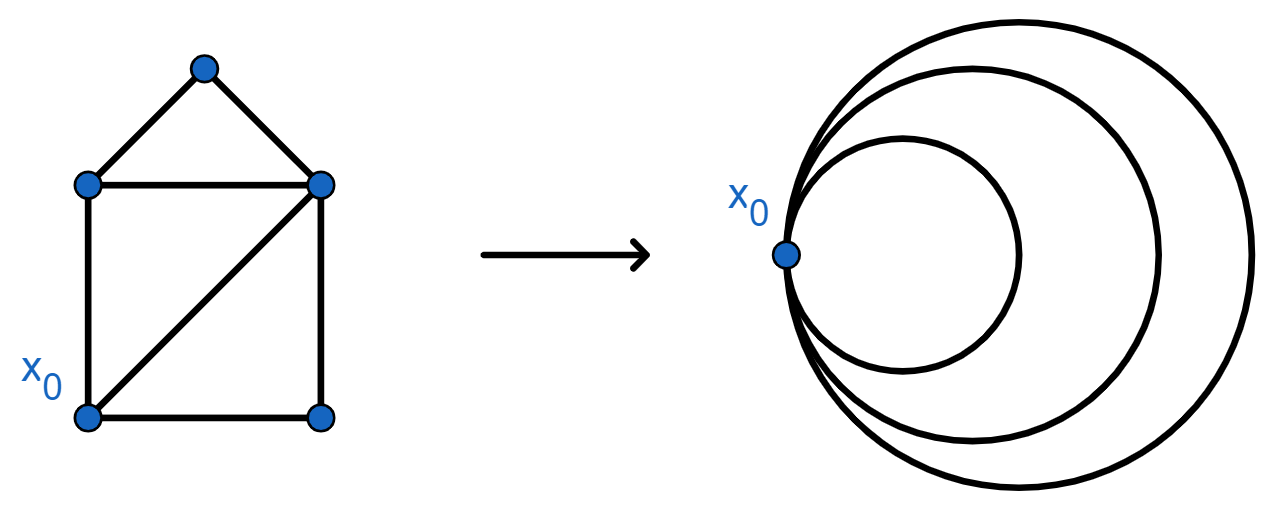
\includegraphics[width=0.55\linewidth]{v3.png}
    \end{figure}
    \begin{figure}[h]
        \centering
        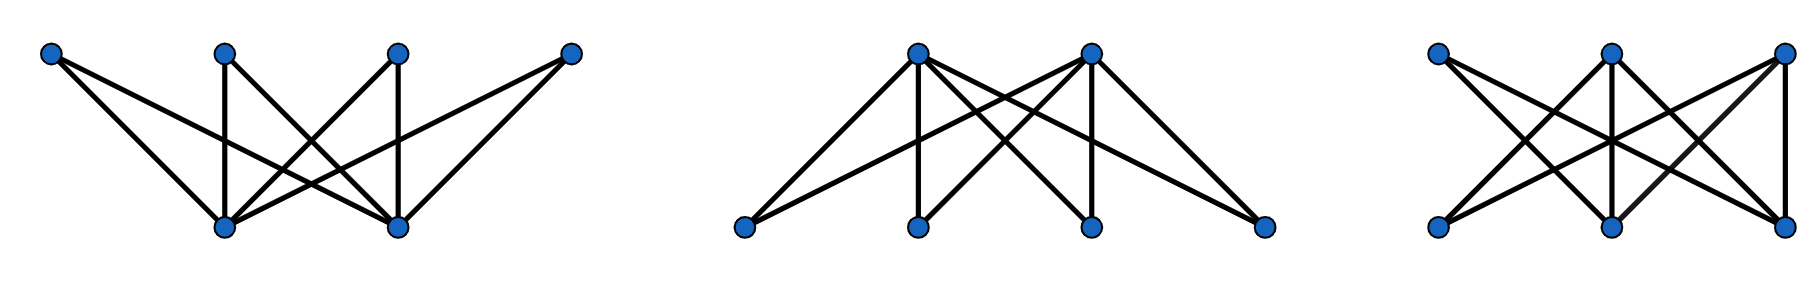
\includegraphics[width=0.8\linewidth]{grafi.png}
    \end{figure}

    Graf na sliki ima eulerjevo karakteristiko enako $-2$, zato je homotopsko ekvivalenten šopu $3$ krožnic, $\bigvee\limits_{i=1}^{3}S^1$. Vsak model za $\bigvee\limits_{i=1}^{3}S^1$ ima $6$ točk in $8$ robov. Ker obstajajo trije nehomeomorfni končni prostori s temi lastnosti vidimo, da graf v splošnem nima enolično določenega minimalnega modela.
\end{primer}

\section*{Slovar strokovnih izrazov}


\geslo{edge path}{lomljenka}
\geslo{edge path group}{grupa sklenjenih lomljenk}
\geslo{down set}{navzdol zaprta množica}
\geslo{Euler characteristic}{Eulerjeva karakteristika}
\geslo{homotopy equivalence}{homotopska ekvivalenca}
\geslo{join}{spoj}
\geslo{simplicial complex}{simplicialni kompleks}
\geslo{up set}{navzgor zaprta množica}
\geslo{weak homotopy equivalence}{šibka homotopska ekvivalenca}
\geslo{wedge sum}{šop}
\geslo{$\h-$path}{\pot}


% seznam uporabljene literature
\begin{thebibliography}{99}

\bibitem{spanier}
E.H.~Spanier, \emph{Algebraic topology}, Springer, New York, 1995.

\bibitem{barmak}
J.A.~Barmak, \emph{Algebraic topology of finite topological spaces and applications}, Lecture notes in mathematics, Springer, Berlin, 2011.

\bibitem{hatcher}
A.~Hatcher, \emph{Algebraic topology}, Cambridge Univ. Press, Cambridge, 2002.



\end{thebibliography}

\end{document}


